% This paper can be formatted using the % (instead of conference) mode.
%++++++++++++++++++++++++++++++++++++++++++++++++++++++
%\documentclass[conference]{IEEEims} % Modified for MTT-IMS
%\documentclass[conference]{IMSTemplate}
\documentclass[conference]{IEEEtran}
%++++++++++++++++++++++++++++++++++++++++++++++++++++++


%+++++++++++++++++++++++++++++++++++++++++++
% Added to commands
\input epsf
\usepackage{graphicx}
\usepackage{amsfonts}
\usepackage{mathtools}
\usepackage{amssymb}
\usepackage{amsmath}
\usepackage{amsthm}
\usepackage{float}
\usepackage{verbatim} %use for comment
\newtheorem{prop}{Proposition}
\newtheorem{theorem}{Theorem}
%+++++++++++++++++++++++++++++++++++++++++++
% correct bad hyphenation here
\hyphenation{op-tical net-works semi-conduc-tor IEEEtran}
\begin{document}
    
    \title{\LARGE v.0306}
    \author{Gioele Migno, Filippo Ficarola, Leonardo Pio Lo Porto}
    % make the title area
    \maketitle
    
    \begin{abstract}
abstract test Leo
\end{abstract}


%\IEEEoverridecommandlockouts
%\begin{keywords}
%Ceramics, coaxial resonators, delay filters, delay-lines, power
%amplifiers.
%\end{keywords}
    
    \section{Introduction}
        intro
    
    \section{Theoretical Fundamentals}
        In this section, we will introduce all the theoretical fundamentals necessary to understand the theory behind the Hamilton-Jacobi Reachability Analysis.

\subsection{Reachability Analysis}
The goal of reachability analysis is to compute the reach-avoid set (RAS) defined as the set of initial states from which the system, using an optimal input, can be driven to a target set within a finite time horizon and satisfying time-varying state constraints at all times. In a reachability problem formulation, the target set can represent a set of undesired states (unsafe), or a set of desired states, in the first case, the RAS contains states to avoid since there exists an optimal input (disturbance) that leads the state into an unsafe region. In the second case instead, the RAS represents safe states from which, applying an optimal input (control law), the system can reach a desired state. 
In the literature, the just described reach-avoid set, is also called capture basin \cite{new_paper} or backward reachable set (BRS) \cite{brief_intro}. In alternative to it, in some cases one might be interested in computing a forward reachable set (FRS), defined as the set of all states that the system can reach from a given initial set of states after a finite time horizon. To understand the difference between BRS and FRS, consider a reachability problem in which the target set contains unsafe states, the FRS can be used to check whether the set of possible future states of the system includes undesired states, the BRS instead, can be used to compute, by starting from known unsafe conditions, those initial states that must be avoided. In this paper HJ-RA is used to compute the BRS of the system, however, it can be used also to compute the FRS. 
All systems in the real world are subject to a disturbance, hence they have two different kinds of inputs, a controllable one $u$ (control) and another uncontrollable $d$ (disturbance); for that reason the computation of the BRS can be formulated in terms of a two-player game. For instance, consider an aircraft that has to follow a trajectory to complete a task, the system has two inputs: a control input (Player 1) and a disturbance (Player 2), in this scenario, the disturbance could be the wind. Suppose now that there is a goal position to reach (target set) along the trajectory, therefore the control input tries to bring the state at the target and the disturbance to steer it away, in this case, the BRS contains all the initial states for which exists an optimal control command that despite the worst disturbance, brings the system at the goal position. Suppose instead of a goal, there is an obstacle along the trajectory, now the target set is defined by all states of the system that correspond to a collision with the obstacle, therefore, the BRS contains those states which could lead to a collision despite the best possible control action. In both cases, the BRS can be computed by studying the outcome of the game between the two players. Due to the way they are formulated, those two games are “games of kind”, namely games in which the outcome is binary: system reaches or not the target set. In order to solve this type of game, it is necessary to translate it into a “games of degree” in which players want to optimize a cost function $J(\cdot)$, with opposite goals: one tries to maximize and the other to minimize it. An approach we will see later, called Level Set Method, can perform this kind of transformation by translating the problem into a standard differential game.

\subsection{Differential Games}
In this section we will introduce the basic concepts of the game theory related to a two person, zero-sum differential game, namely a mathematical representation in game theory of a situation which involves two sides, where the result is an advantage for one side and a loss for the other. If the total gains of the participants are added up, and the total losses are subtracted, they will sum to zero.
\newline
\subsubsection{Definition of the differential game}
Consider the system dynamics $\dot{x}=f(x(s), u(s), d(s))$ where $s \in [t, T]$ represents the time variable, $x(\cdot)\in\mathbb{R}^n$, $u(\cdot)\in U\subseteq \mathbb{R}^m$, $d(\cdot)\in D\subseteq \mathbb{R}^p$, $f:\mathbb{R}^n \times U \times D \rightarrow \mathbb{R}^n$. We use $s$ as the time variable to agree with the standard notation in game theory in which the game starts at time $s=t$ and ends at $s=T$ \cite{evans}.
The inputs $u(\cdot)$, $d(\cdot)$ represent Player 1 (control) and Player 2 (disturbance) respectively, we assume that they are drawn from the set of measurable functions \cite{evans}\cite{brief_intro}:
\[ 
    u(\cdot) \in \mathcal{U}_{[t, T]}  \triangleq 
    \left\{
        \sigma: [t, T] \rightarrow U| \sigma(\cdot) \, \textrm{is measurable} \, 
    \right\} 
\]
\[ 
    d(\cdot) \in \mathcal{D}_{[t, T]}  \triangleq 
    \left\{
        \sigma: [t, T] \rightarrow D| \sigma(\cdot) \, \textrm{is measurable} \, 
    \right\} 
\]
Assume $U$, $D$ are compact, $f(\cdot)$ is bounded and Lipschitz continuous in $x(\cdot)$ and continuous in $u(\cdot)$ and $d(\cdot)$, therefore, the system dynamics admits an unique trajectory $x(\cdot)$ that represents the response of the system to the inputs $u(\cdot)$, $d(\cdot)$ starting from an initial state $x(t)=x$.
The differential equation associated to the game is then the following one:
\begin{equation}
	\label{ode}
	\left\{
		\begin{array}{ll}
			\dot{x}(s)=f(x(s), u(s), d(s))  & s \in [t, T] \\
			x(t) = x
		\end{array}
	\right.
\end{equation}

In order to complete the game definition is necessary to introduce the payoff function of the game $J(\cdot)$ and to do that we use two Lipschitz continuous functions $c:\mathbb{R}^n \rightarrow \mathbb{R}$ and $q:\mathbb{R}^n \rightarrow \mathbb{R}$:
\begin{equation}
	\label{payoff}
	J(x, t, u(\cdot), d(\cdot)) = \int_{t}^{T} c(x(s),d(s),u(s),s)  \,ds + q(x(T)) 
\end{equation}

The payoff function represents the reward/cost obtained by the two players at the end of the differential game (\ref{ode}) started at time $t$ with an initial state $x$, and subject to the commands  $u(\cdot)$, $d(\cdot)$ chosen by Player 1 and Player 2 respectively. The function $c(\cdot)$ indicates a running cost, therefore the first term of (\ref{payoff}) is the reward gained during the game (trajectory). The second term instead, uses $q(\cdot)$ to evaluate the final state $x(T)$ reached.
\newline

\subsubsection{Value of the game}
In order to solve the game, namely computes its outcome, it's necessary to define the goal and the information pattern of each player. Since we are referring to a zero-sum game, the aims of the players must be opposite, without loss of generality we assume Player 1 ($u(\cdot)$) wants to minimize the cost function $J(\cdot)$ and Player 2 ($d(\cdot)$) tries to maximize it. The information pattern of a game indicates which information a player has respect to its opponent.

In the case of simple games, usually there exists a dominant strategy for each player, namely an optimal strategy that is better than other ones independently to the opponent's strategy. In these cases it is easy to solve the game, since assuming rational players, we know a priori the strategies that will be chosen and therefore we can compute the game outcome in advance. In more complex games like the differential game (\ref{ode}) in which no longer exists dominant strategies, we cannot predict the outcome therefore we have to find another way to solve the game. For this reason in game theory two quantities called lower value $V^-(\cdot)$ and upper value $V^+(\cdot)$ are defined. The lower value $V^-(\cdot)$ indicates the lowest possible outcome of the game (the lowest value of $J(\cdot)$), the upper value $V^+(\cdot)$ is instead the highest one, these values can be defined by giving to a player an advantage respect to the other one. As done in \cite{evans} \cite{reach_avoid_with_dist} \cite{brief_intro} to give a strategic advantage to a player, we impose to him the use of a non-anticipative strategy. This is an advantage because during the game, we assume that each player can choose its own input by knowing the current state of the system (system feedback), and in addition to this information, if a player can use a nonanticipative strategy then it knows also the current input chosen by its opponent \cite{mitchell_time_dep_HJ}.

The lower value of the game is defined by giving to the player that wants to minimize the cost function $J(\cdot)$ the strategic advantage, therefore we define a nonanticipative strategy for $u(\cdot)$ in the following way \cite{evans}:

\begin{equation}
	\label{eq:non_ant_stra_u}
	\begin{split}
		\gamma \in \Gamma \triangleq 
		& \left\{ 
			\alpha : \mathcal{D}(t) \rightarrow \mathcal{U}(t)\,|\,d(r) = \hat{d}(r) \in \mathcal{D}(t)
		\right. \\ 
		& \textrm{for almost every} \;r \in [t,s] \\
		& \implies \alpha[d](r)= \alpha[\hat{d}](r) \\
		& \left. 
			\textrm{for almost every} \; r \in [t,s] 
		\right\}  
	\end{split}
\end{equation}

What the formula says is that, a map $\alpha : \mathcal{D}(t) \rightarrow \mathcal{U}(t)$ is a nonanticipative strategy if for any $s \geq t$, for any $d(\cdot)$ and $\hat{d}(\cdot)$ belonging to $\mathcal{D}$ such that $d(\cdot)$ and $\hat{d}(\cdot)$ coincide almost everywhere on $[t,s]$, the image $\alpha(d(\cdot))$ and $\alpha(\hat{d}(\cdot))$ coincide almost everywhere on $[t,s]$ This restriction means that if player 1 cannot distinguish between input signals $ \alpha (d( \cdot )) $ and $ \alpha (\hat{d}( \cdot ) )$ of player 2 until after time $s$, then player 1 cannot respond differently $( \alpha [d](r) = \alpha [\hat{d}](r))$ to those signals until after time $s$. Or in other words, player 1 cannot respond differently to two different player 2 disturbances until they become different.

Now we can define the lower value of the game $V^-(x,t)$ by allowing $u(\cdot)$ to use $\gamma(\cdot)$:
\begin{equation}
	\label{lower_value_game}
	V^-(x,t) \triangleq \inf_{\gamma(\cdot) \in \Gamma(\cdot)}\sup_{d(\cdot) \in \mathcal{D}(\cdot)}J(x,t, \gamma[d](\cdot), d)
\end{equation}

As mentioned before, in general $V^-(x,t)$ is not the outcome but represents the lower outcome possible of the game started at time $t$ with initial state $x$. However, it is important to highlight that if we assume the use of the information pattern just described (Player 1 uses nonanticipative), then $V^-(x,t)$ is the actual outcome of the game.

Similarly we can define the upper value of the game $V^+(x,t)$, this time Player 2 ($d(\cdot)$) uses a nonanticipative strategy defined as:
\begin{equation}
	\label{eq:non_ant_stra_d}
	\begin{split}
		\delta \in \Delta \triangleq 
		& \left\{ 
			\alpha : \mathcal{U}(t) \rightarrow \mathcal{D}(t)\,|\,u(r) = \hat{u}(r) \in \mathcal{U}(t)
		\right. \\ 
		& \textrm{for almost every} \;r \in [t,s] \\
		& \implies \alpha[u](r)= \alpha[\hat{u}](r) \\
		& \left. 
			\textrm{for almost every} \; r \in [t,s] 
		\right\}  
	\end{split}
\end{equation}

The upper value is then defined by giving to $d(\cdot)$ (player that wants maximizes $J(\cdot)$) the strategic advantage:
\begin{equation}
	\label{upper_value_game}
	V^+(x,t) \triangleq \sup_{\delta(\cdot) \in \Delta(\cdot)}\inf_{u(\cdot) \in \mathcal{U}(\cdot)} J(x,t, u, \delta[u](\cdot))
\end{equation}

For theroretical completeness, we note that $V^-(x,t) \leq V^+(x,t)$ for any $(x,t)$. In those cases in which equality holds, the game is said to have value and $V(x,t)\triangleq V^-(x,t) = V^+(x,t)$ is called the value of the game. \cite{new_paper} \newline

\subsubsection{Differential Game in Reachability Analysis}
Let's try now to understand how differential games theory is related to a reachablity problem, to do that assume we are in the case in which we have a set to reach, namely the target set is a desired set of states. In this case Player 1 tries to bring the system towards the target with its input $u(\cdot)$ and in the meanwhile the disturbance (Player 2) tries to steer the system away the target with its input $d(\cdot)$. This problem can be through as a game between the two players, however in this form, the game theory just described cannot be used since the reward function is a simple boolean value: at the end of the game the system state reaches (Player 1 wins) or not the target set, so we have $J(\cdot)=\left\{0 \textrm{ (win)},1\textrm{ (loss)}\right\}$. To solve this issue we can easily use the Level Set Method that allows to rewrite $J(\cdot)$ as a real function, we will see this later. For the moment assume Player 1 wants to minimize a real value function $J(\cdot)$ and Player 2 tries to maximize it. 
Now we have to understand why the lower and the upper value of the game are important for our purpose. As said before, $V^-(x,t)$ or $V^+(x,t)$ is the actual outcome of the game only if we give a strategic advantage to one player, therefore introducing an information pattern for our game, we can easily define formally the outcome through one of them. In order to consider always the worst possible scenario, the strategic advantage is usually given to the disturbance $d(\cdot)$, then since its aim is to maximize the cost function, the outcome of the game is defined by $V^+(x,t)$.
In a different scenario in which $u(\cdot)$ maximizes and $d(\cdot)$ minimizes $J(\cdot)$ then, since the strategic advantage must be assigned to the disturbance, the outcome this time is given by $V^-(x,t)$. In this paper we always refer to the first scenario. 

As we will see later the BRS is related to the outcome of the game ($V^+(x,t)$), this allows us to solve our reachability problem using the upper value of the game. 
One important result of dynamic programming is that the value functions $V^\pm(x,t)$ are the viscosity solutions of two particular variational inequalities in the form of a Hamilton-Jacobi-Isaacs equation. We will see this formally later, let's now introduce what is a HJI equation, a viscosity solution and how to use the Level Set Method.

\subsection{Hamilton-Jacobi Equation}					
In physics, the Hamilton-Jacobi equation is an alternative formulation of classical mechanics. It is a first-order nonlinear partial differential equation of the form $H(x,u_x(x,\alpha,t),t)+u_t(x,\alpha,t)=K(\alpha,t)$ with independent variables $(x,t)\in \mathbb{R}^n \times \mathbb{R}$ and parameters $\alpha \in \mathbb{R}^n$. It has wide applications in many scientific fields like mechanics. Its solutions determine infinite families of solutions of Hamilton's ordinary differential equations, which are the equations of motion of a mechanical system. In our case, the family of solutions that come from the computation of the HJI PDE and the variational inequality is the viscosity solution. 

\subsection{Viscosity Solution}

Viscosity solution is a concept introduced in \cite{vis_sol}; it is a notion of solution that allows it to be, for example, nowhere differentiable but for which strong uniqueness theorems, stability theorems and general existence theorems are all valid. It is a generalization of the solution to a partial differential equation (PDE). It has been found that the viscosity solution is that kind of solution to use in many applications of PDE's, including for example first order equations arising in dynamic programming (the Hamilton–Jacobi–Bellman equation) or differential games (the Hamilton–Jacobi–Isaacs equation). This means that, given the classical concept of PDE 
\begin{equation}
	\label{diff_eq}
	F(y,u(y), Du(y))=0
\end{equation}

Under the viscosity solution concept, a certain variable $u$ does not need to be everywhere differentiable. There may be points where $Du$ does not exist and yet $u$ satisfies the equation in an appropriate generalized sense.

Taking the main concepts of viscosity solutions from \cite{vis_sol}, let $u$ be a function from O into $\mathbb{R}$  and let $y_0$ belong to $\mathcal{O}$.  The superdifferential and subdifferential of $u$ at $y_0$, denoted, respectively, by $D^{+} u(y_0)$ and $D^{-} u(y_0)$ are the set of points for which, respectively, the following two inequalities hold:

\begin{equation}
	\limsup_{y \to y_0} (u(y)-u(y_0)-p_0 \cdot (y-y_0)) |y-y_0|^{-1} \leq 0
\end{equation}
and

\begin{equation}
	\liminf_{y \to y_0} (u(y)-u(y_0)-p_0 \cdot (y-y_0)) |y-y_0|^{-1} \geq 0
\end{equation}

where $p_0 \cdot (y-y_0)$ is the Euclidean scalar product of $p_0$ and $(y-y_0)$. 
Given these concepts it is possible to define what is a viscosity solution mathematically. 
If $D^+u(y_0)$ and $D^-u(y_0)$ are nonempty at some $x$ and $u$ is differentiate at $x$, a viscosity solution of (\ref{diff_eq}) is a function $u$ belonging to $C(\mathcal{O})$ satisfying the two following conditions:

\begin{equation}
	F(y,u(),p)\leq 0 \forall y \in \mathcal{O}, \forall p \in D^+ u(y)
\end{equation}

\begin{equation}
	F(y,u(),p)\geq 0 \forall y \in \mathcal{O}, \forall p \in D^- u(y)
\end{equation}


\subsection{Level Set Method}
As mentioned before, in order to compute the BRS is necessary to solve a game of kind where the outcome is boolean: the system state either reaches the target set or not. Level Set Method can be used to translate this game into a game of degree, where players share an objective function to optimize. The basic idea of this approach is to encode the boolean outcome through a quantitative function $g(\cdot)$ and compare its value at the end of the game to a threshold value, usually zero, to determine whether the system reached the target set.
The first step is to define a Lipschitz function $g(x(\tau))$, where $x(\tau)$ represents the current system state ($s=\tau\in[t, T]$), such that the target set $R$ corresponds to the zero sublevel set of $g(x(\tau))$, that is, $x(\tau)\in R \Leftrightarrow g(x(\tau)) \leq 0$. We indicated the target set with $R$ (reach) since from now on we suppose that the set contains goal states, namely states to reach. Now we can define the real value cost function of the game $J(\cdot)$, we are not interested in any kind of running cost, therefore we consider only the value of $g(\cdot)$ at the end of a game started at time $s=t$ and initial state $x$:

\begin{equation}
\label{eq:j_level_set}
    J(x, t, u(\cdot), d(\cdot)) = g(x(T))
\end{equation}

Assuming our reachability problem consists only of reaching a target set $R$, then the goal of our control input $u(\cdot)$ is to minimize $J(\cdot)$ while the disturbance $d(\cdot)$ tries to do the opposite. Then giving the strategic advantage to $d(\cdot)$, namely force it to use the non-anticipative strategy $\delta[d](\cdot)$, we define the outcome of the game through its upper value:
\begin{equation}
	\begin{split}
		V^+(x, t) 
		& = \sup_{\delta(\cdot) \in \Delta(\cdot)}\inf_{u(\cdot) \in \mathcal{U}(\cdot)} J(x,t, u, \delta[u](\cdot))    \\
		& = \sup_{\delta(\cdot) \in \Delta(\cdot)}\inf_{u(\cdot) \in \mathcal{U}(\cdot)} g(x(T))
	\end{split}
\end{equation}

However, in practical scenarios, along the trajectory of a dynamical system there may be both goals to reach and obstacles to avoid. The goals to reach can be represented by the target set $R$ as previously done, the set of states to avoid instead, can be defined with another set $A$ (avoid) that contains all the system state $x$ that corresponds to an object collision. This kind of formulation is adopted in \cite{reach_avoid_with_dist} however, we will use another one from \cite{new_paper} in which instead of $A$, its complementary set $K$ is defined. This choice is due to the fact that \cite{new_paper} provides a more advanced problem formulation allowing sets $R$ and $K$ to be time-varying, namely allows to define a reachability problem in which both the goals and the obstacles can vary their positions over time. According to this new formulation, since $R$ can vary over time, also the function $g(\cdot)$ must be time-dependent. The new set $K$ is characterized similarly to $R$ by intoducing another function $h(\cdot)$. Formally: consider the sets $R$, $K$ related respectively to the level sets of two Lipschitz continuous and bounded functions $g: \mathbb{R}^n \times s \in [t, T]\rightarrow \mathbb{R}$, $h: \mathbb{R}^n \times s \in [t, T] \rightarrow \mathbb{R}$, then the two sets can be characterized as:

\begin{equation} 
	\label{R}
	R = \left\{ (x,s) \in \mathbb{R}^n \times [t,T]\,|\, g(x, s) \leq 0 \right\}
\end{equation}
\begin{equation} 
	\label{K}
	K = \left\{(x,s) \in \mathbb{R}^n \times [t,T] \,|\, h(x, s) \leq 0 \right\}
\end{equation}

The most common choice for the functions $g(\cdot)$ and $h(\cdot)$ is to use the distance between the current state $x$ and the set of interested, namely:

\begin{equation}
\label{g}
    g(x, s) =
\left\{
	\begin{array}{ll}
		-d(x, s, R^c)  & \mbox{if } x \in R \\
		d(x, s, R) & \mbox{if } x \in R^c
	\end{array}
\right.
\end{equation}

\begin{equation}
\label{h}
    h(x, s) =
\left\{
	\begin{array}{ll}
		-d(x, s, K^c)  & \mbox{if } x \in K \\
		d(x, s, K) & \mbox{if } x \in K^c
	\end{array}
\right.
\end{equation}

Since $g(\cdot)$, $h(\cdot)$ must be bounded, we will see later why, we can introduce two constants $C_g$ $C_h$ to impose a saturation to the distance functions, or alternatively, we can use the arctangent of the signed distance, in this way the resulting functions are bounded and also globally Lipschitz \cite{reach_avoid_no_dist}. 

In the next section we will see how the value function $V^+(\cdot)$ is formulated when we have both a reach $R$ and a constraints $K$ set, and most importantly how it can be computed in order to calculate the BRS. In the following sections we will refer to the BRS as a reach-avoid set (RAS) to highlight the fact that there is both a set to reach and one to avoid, this last is implicity defined by its complementary $K$, namely $A \triangleq K^c$.

    
    \section{Computation Reach-Avoid set}
        In this section we will see how all the previous theoretical concepts can be applied to solve a reachability problem, in which the system state has to reach a desired set $R$ while remains in the constraints set $K$ that represents the complementary of the set of states $A$ that correspond to a collision between the system and an obstacle in the real world.

Given the previous specifications, we can define two different kinds of reachability problems. In the first one we are interested in reaching safely $R$ exactly at the end of the game $(s=T)$, in the second instead, the system can reach safely $R$ at any $s$ inside the time horizon $[t, T]$. In the following we will focus our attention only on this last one.

Consider the system dynamics (\ref{ode}), the two functions $g(\cdot)$, $h(\cdot)$ defined in (\ref{g})(\ref{h}) and used to represent the target set $R$ and the constraint set $K$ respectively. As said before, under these conditions, the system dynamics admits a unique trajectory $x(s)$ from an initial state $x$ at time $t$ under inputs $u(\cdot)$ and $d(\cdot)$. We denote this solution as:
\[
    \phi(s; x, t, u(\cdot), d(\cdot)) : [t, T] \rightarrow \mathbb{R}^n
\]

\subsection{Payoff Function}
We have already seen the payoff function of a reachability problem in which there is only a set to reach (\ref{eq:j_level_set}), now we have to consider also the constraints set $K$ and to do that we can use the following cost function \cite{new_paper}:
\begin{equation}
    \label{j_ras}
    J(x, t, u(\cdot), d(\cdot)) =  
        \min_{\tau \in [t, T]}
        \left\{
            \mathcal{J}(\tau, x, t, u(\cdot), d(\cdot))
        \right\}
\end{equation}
\begin{equation}
    \label{jj_ras}
    \mathcal{J}(\tau, x, t, u(\cdot), d(\cdot)) =  
        \max
        \left\{
            g(\mathcal{X}(\tau), \tau), \max_{r \in [t, \tau]}h(\mathcal{X}(\tau), r)            
        \right\}
\end{equation}
Where: 
\[\mathcal{X}(\tau)=\phi(\tau; x, t, u(\cdot), d(\cdot))\]

The $J(\cdot)$ function is used to evaluate the game and therefore determines if Player 1 ($u(\cdot)$) won or lost. The expression (\ref{j_ras}) considers the value of another function $\mathcal{J}(\cdot)$ for all time $\tau \in [t, T]$ during the game. For each instant $\tau$, $\mathcal{J}(\cdot)$ takes the maximum between two quantities, the first one uses $g(\cdot)$ to determine if the current system state is inside the reach set $R$ and the second instead, uses $h(\cdot)$ to check whether or not the state had ever left the constraints set $K$ so far, namely on time interval $[t, \tau]$. The maximum value of $h(\cdot)$ is taken in order to keep in mind a previous collision before $\tau$, indeed we recall that $(x,s) \in K \Leftrightarrow h(x,s) \leq 0$, therefore a positive value of $h(\cdot)$ indicates an exit from $K$ (obstacle collision).
So, for a given $\tau \in [t, T]$, we have $\mathcal{J} \leq 0$ if and only if, the system trajectory started at time $t$ with initial state $x$, reaches the target $R$ at time $\tau$ without ever having collided with an obstacle on $[t, \tau]$, if this situation takes place for any $\tau \in [t, T]$ then Player 1 wins. For that reason, $J(\cdot)$ takes the minimum time $\tau$, in this way the control input $u(\cdot)$ can win at any moment during the game. It is important to highlight that $J(\cdot)$ does not take into account any collision after the system reached the target set $R$. 

Once defined the cost function of the game, $V^-(x,t)$ and $V^+(x,t)$ are defined in the same way of (\ref{lower_value_game}) (\ref{upper_value_game}) respectively.

\subsection{Definition Reach-Avoid Set}
We are finally ready to define formally the RAS. As said before, we assume $u(\cdot)$ tries to minimize the distance of the system state to $R$, and $d(\cdot)$ tries to do the opposite, potentially also bringing the state outside the constraints set $K=A^c$. In order to consider the worst possible case, we give the strategic advantage to the disturbance, in this way the outcome of the game is given by $V^+(x,t)$ and using it we can compute $RAS^+$. For completeness, we also report the definition of $RAS^-$ namely the reach-avoid set computed through the lower value of the game $V^-(x,t)$.

Given an information pattern, we define the reach-avoid set as the set of point $(x,t)$ for which the system trajectory $\phi(\cdot)$, starting at time $t$ with initial state $x$ and both players acting optimally, reaches the target set $R$ at some instant $\tau \in [t, T]$ while remaining inside the constraints set $K$ for all $s \in [t, \tau]$. We indicate with $\mathcal{R}_s$, $\mathcal{K}_s$ the target set $R$ and the constraints set $K$ at time $s$ respectively.

When the strategic advantage is given to the player that wants to maximize the outcome ($d(\cdot)$), we indicate the reach-avoid set with $RAS^+$ that is formally defined as \cite{new_paper}:
\begin{multline}
    \label{ras_p}
    RAS^+ = 
    \left\{
        (x,t) \in \mathbb{R}^n \times [0,T] \,|\, \exists u^*(\cdot) \in \mathcal{U}_{[0, T]},
    \right.\\
    \left.
          \forall \delta(\cdot) \in \Delta_{[0, T]}, \exists \tau \in [t, T], \phi(\tau; x, t, u^*(\cdot), \delta(\cdot)) \in \mathcal{R}_\tau \quad \wedge \quad       
    \right.\\
    \left.
        \forall s \in [t, \tau], \phi(s; x, t, u^*(\cdot), \delta(\cdot)) \in \mathcal{K}_s
    \right\}
\end{multline}

Similarly, when the player that tries to minimize uses a nonanticipative strategy:
\begin{multline}
    \label{ras_m}
    RAS^- = 
    \left\{
        (x,t) \in \mathbb{R}^n \times [0,T] \,|\, \exists \gamma^*(\cdot) \in \Gamma_{[0, T]},
    \right.\\
    \left.
          \forall d(\cdot) \in \mathcal{D}_{[0, T]}, \exists \tau \in [t, T], \phi(\tau; x, t, \gamma^*(\cdot), d(\cdot)) \in \mathcal{R}_\tau \quad \wedge \quad       
    \right.\\
    \left.
        \forall s \in [t, \tau], \phi(s; x, t, \gamma^*(\cdot), d(\cdot)) \in \mathcal{K}_s
    \right\}
\end{multline}
These two formulations of the reach-avoid set are related to the outcome of the game through the following proposition \cite{new_paper}:
\begin{prop}
    \label{ras_p_m_v}
    The reach-avoid set $RAS^\pm$ is given by the zero sublevel set of the game's outcome: 
    \[
        RAS^\pm=
        \left\{
            (x, t) \in \mathbb{R}^n \times [0, T] \,|\, V^\pm(x,t) \leq 0
        \right\}
    \]
\end{prop}
These two reach-avoid sets are related, indeed the reach-avoid set computed when the strategic advantage is given to the disturbance it is a subset of the one computed given the advantage to the control input \cite{new_paper}:
\begin{equation}
    RAS^+ \subseteq RAS^-
\end{equation}
This relation is the reason why we have chosen to give the advantage to the disturbance, in this way we increase the safety margin.

\subsection{Hamilton-Jacobi-Isaacs Equation}
Given an information pattern, the reach-avoid set $RAS^\pm$ is described by the zero sublevel of the game's outcome $V^\pm(x,t)$. This last is the viscosity solution of a specific Hamilton-Jacobi-Isaacs equation \cite{new_paper}:
\begin{theorem}
    Assume $f(\cdot)$ defined as done in (\ref{ode}), $g(x,t)$, $h(x,t)$ globally Lipschitz continuous. Then the value function $V^\pm(x,t)$ is the unique viscosity solution of the following variational inequality in the form of a Hamilton-Jacobi-Isaacs equation:
    \[
        \max
        \left\{
            \mathcal{H}, \Delta h
        \right\} = 0
    \]
    \[
        \mathcal{H} \triangleq \min
        \left\{
            \frac{\partial V^\pm(x,t)}{\partial t} + 
            H^\pm\left(x, \frac{\partial V^\pm(x,t)}{\partial x}, t\right), \Delta g
        \right\} 
    \]
    \[
        \Delta h \triangleq h(x,t) - V^\pm(x,t), \quad \Delta g \triangleq g(x,t) - V^\pm(x,t)
    \]
    \[
        t \in [0, T] \quad x \in \mathbb{R}^n
    \]
    with terminal condition
    \[
        V^\pm(x,T) = \max \left\{ g(x,T), h(x,T) \right\} \quad x \in \mathbb{R}^n
    \]
    The upper and lower Hamiltonians $H^\pm$ are given by:
    \[
        H^+(x,p,t) = \min_{u \in U}\max_{d \in D} p^T f(x, u, d)
    \]    
    \[
        H^-(x,p,t) = \max_{d \in D}\min_{u \in U} p^T f(x, u, d)
    \]
    %where:
    %\[
    %    p = \nabla V(x(t),y(t),\theta(t),t) = [p_{x},p_{y},p_{\theta }] 
    %\]
    \label{th:vis_sol}
\end{theorem}

The algorithm of the numerical method able to compute the value function $V^\pm(x,t)$ in Th. \ref{th:vis_sol} is described in \cite{new_paper}. Please notice here we use different notations for target and constraints functions.

    \section{Case of Study}
        case of study

    \section{Simulation}
        In all simulations, $L=1$, control input $u$ is limited in $U = [-\overline{u}, +\overline{u}]$ where $\overline{u}=1.5$ and the disturbance $d$ in $D=[-\overline{d}, +\overline{d}]$ where $\overline{d}=0.15$. In order to take into account robot dimensions in the configuration space ($\mathcal{C}$-space), we approximate its shape as a circle of $radius = (4/3)L$.

Our Simulations are divided in two main cases: 
\begin{itemize}
    \item The first one takes place in a static environment, where we have fixed obstacles and a fixed target set 
    \item The second one takes place in a dynamic environment with moving obstacles and a moving target set.
\end{itemize}
The second case contains three sub-cases:  
\begin{itemize}
    \item The Robot starts near the target set
    \item The Robot starts distant from the target set
    \item The Robot starts outside the $RAS$ (Reach-Avoid Set)
\end{itemize}
In addiction, for each simulation we test two disturbances strategies: 
\begin{itemize}
    \item Optimal Disturbance (\ref{opt_d})
    \item Random Disturbance 
\end{itemize}
The random disturbance is sampled from a Normal Gaussian distribution, with mean $\mu=0$ and standard deviation $\sigma=\overline{u}/3$. $\sigma$ has this form since in this way most of the samples ($99.7\%$) are in $D$, those outside are clipped.

\subsection{Static Case}
    As mentioned before in this case the robot has to reach a fixed target set wich is among some rectangular fixed obstacles. The simulation develops in a time of 10 seconds.
    We can start seeing the $RAS$ in different instants of time to see its expansion during the regression.
    
    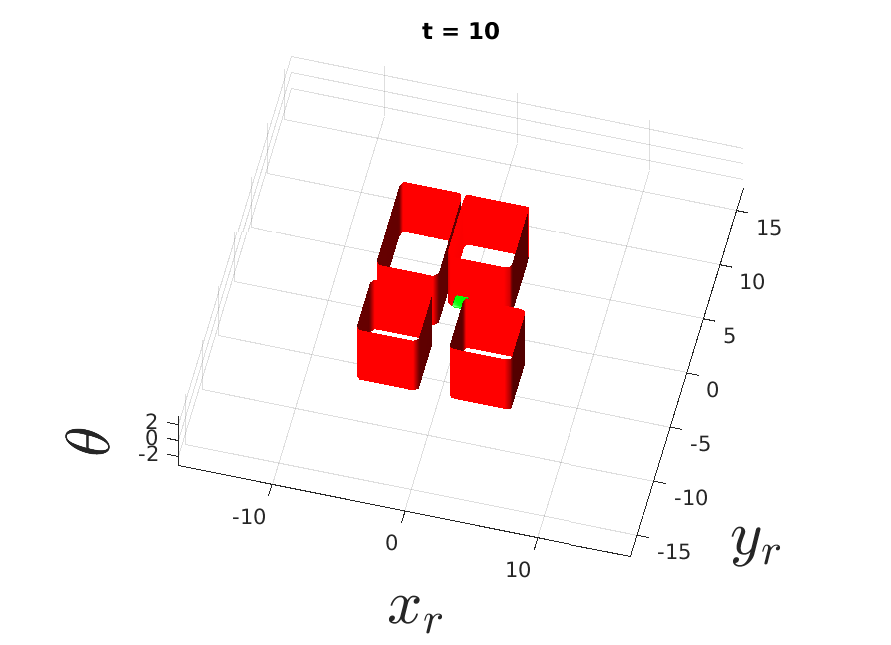
\includegraphics[scale=0.6]{figures/staticRAS1.png}
    
    The 2 horizontal axis represent the X-axis and the Y-xis, while the third one represents the angle Theta: the angle that the X-axis in the robot framework forms with the X-axis of the World Reference Framework.  
    Here we can notice a small green area which represents the target set and 4 red
    rectangles representing the obstacles. Since this representation takes place in the configuration space the obstacles are bigger than their real dimension and the target set seems smaller.
    It is evident from the target set that the robot is not allowed to reach the target set in any possible orientation, but only in a small range around the 0 $rad$ so we expect to see some maneuvers to adjust the orientation.  
    Then we can see the expansion of the $RAS$ to its final limits.
    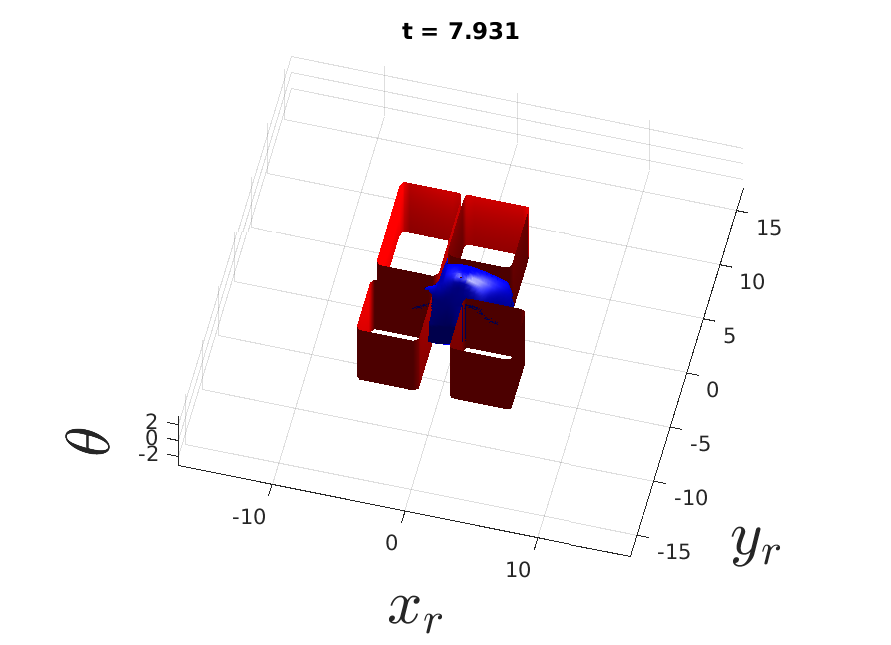
\includegraphics[scale=0.6]{figures/staticRAS2.png}
    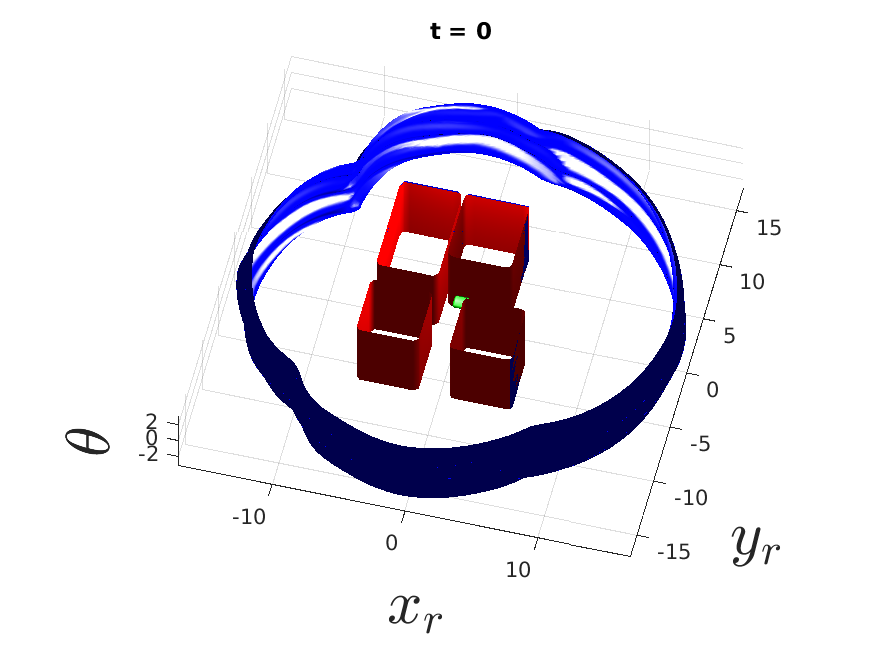
\includegraphics[scale=0.6]{figures/staticRAS3.png}
    The blue area represents the border of the Reach-Avoid Set. So from any initial configuration $(x_{i},y_{i},\theta{i})$ inside the blue border our robot is expected to reach the target set in the time limit of 10 seconds. 
    Now that the $RAS$ is defined we can see how the robot reaches the target set avoiding obstacles and playing against an optimal disturbance.
    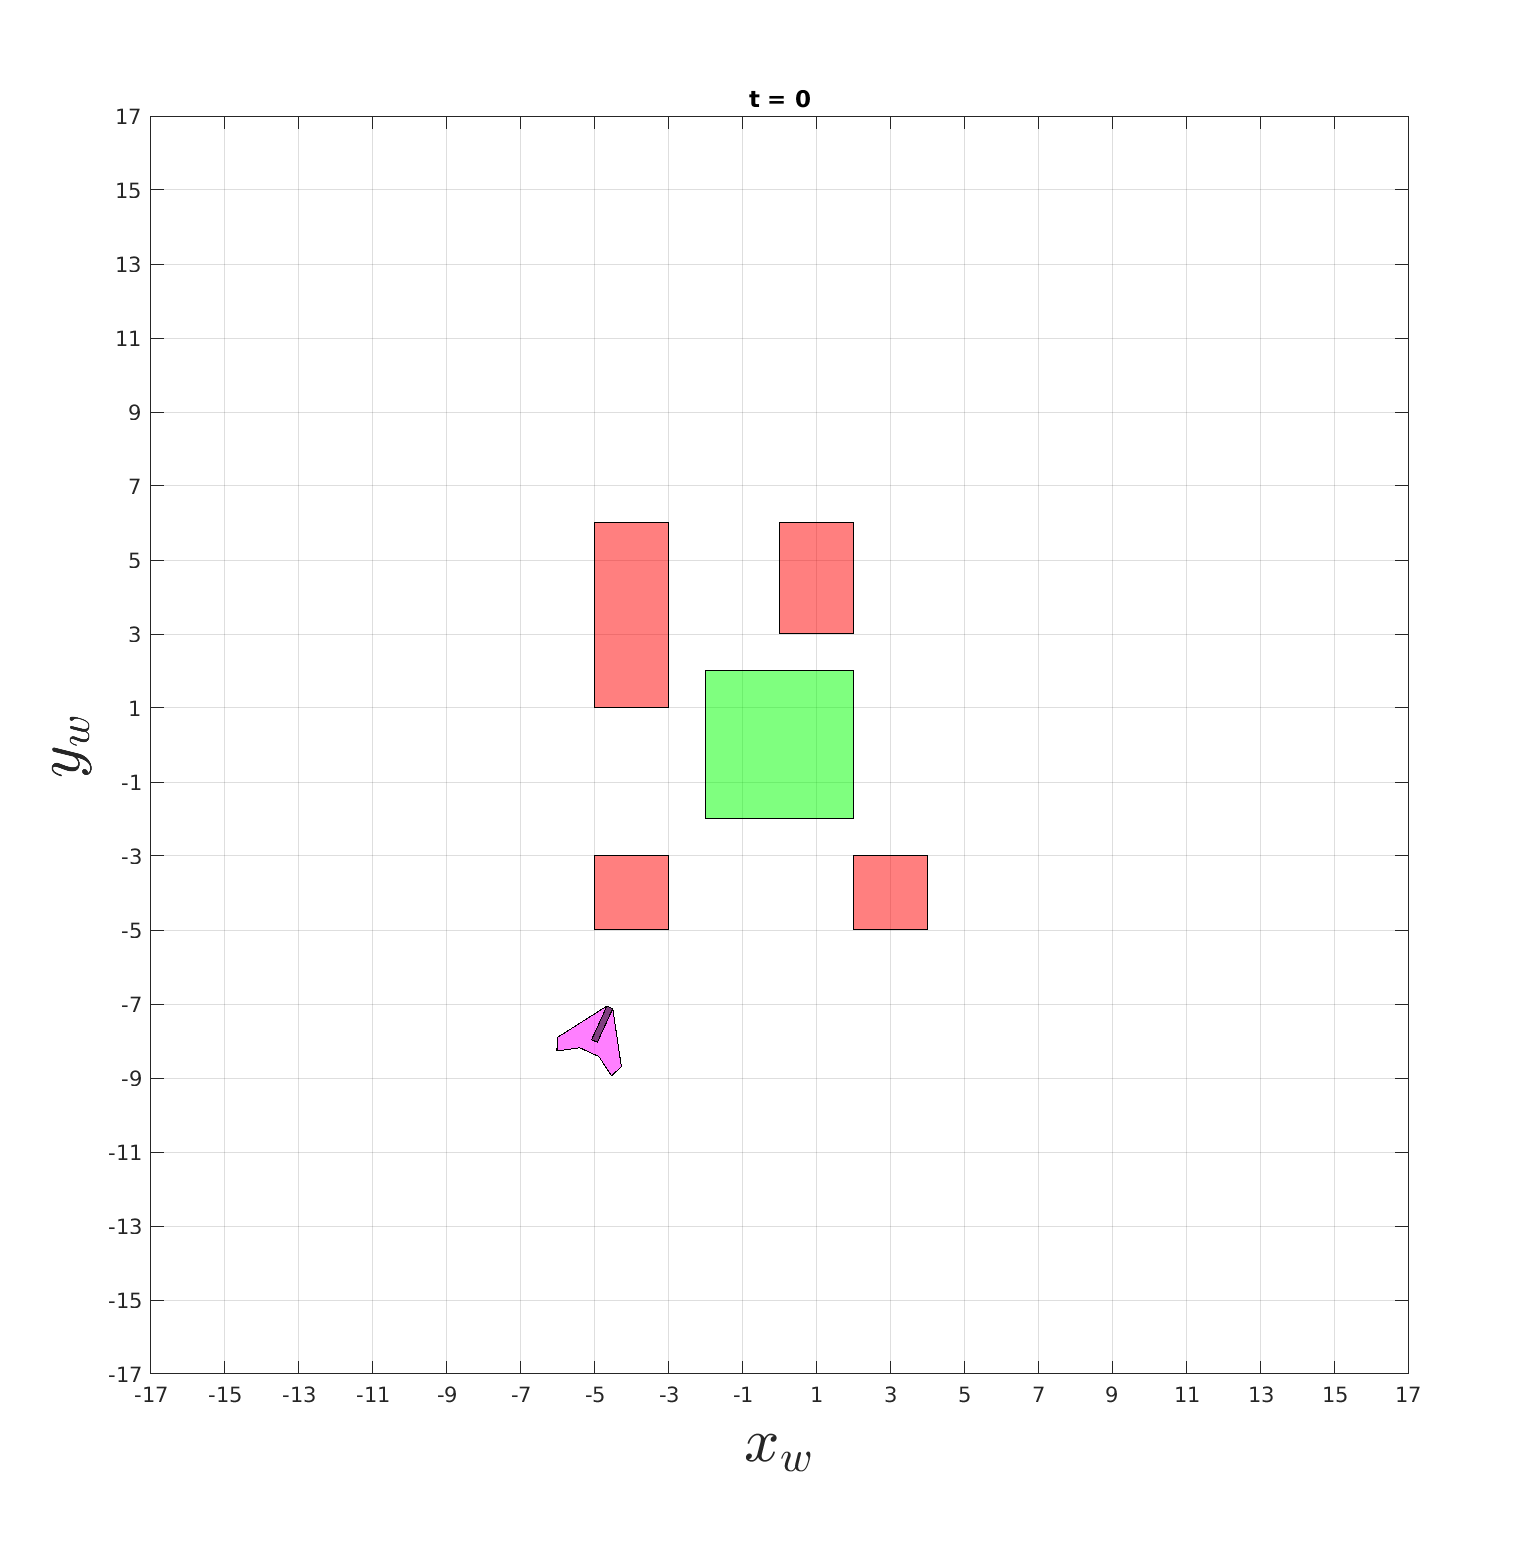
\includegraphics[scale=0.3]{figures/staticTRAJ1.png}
    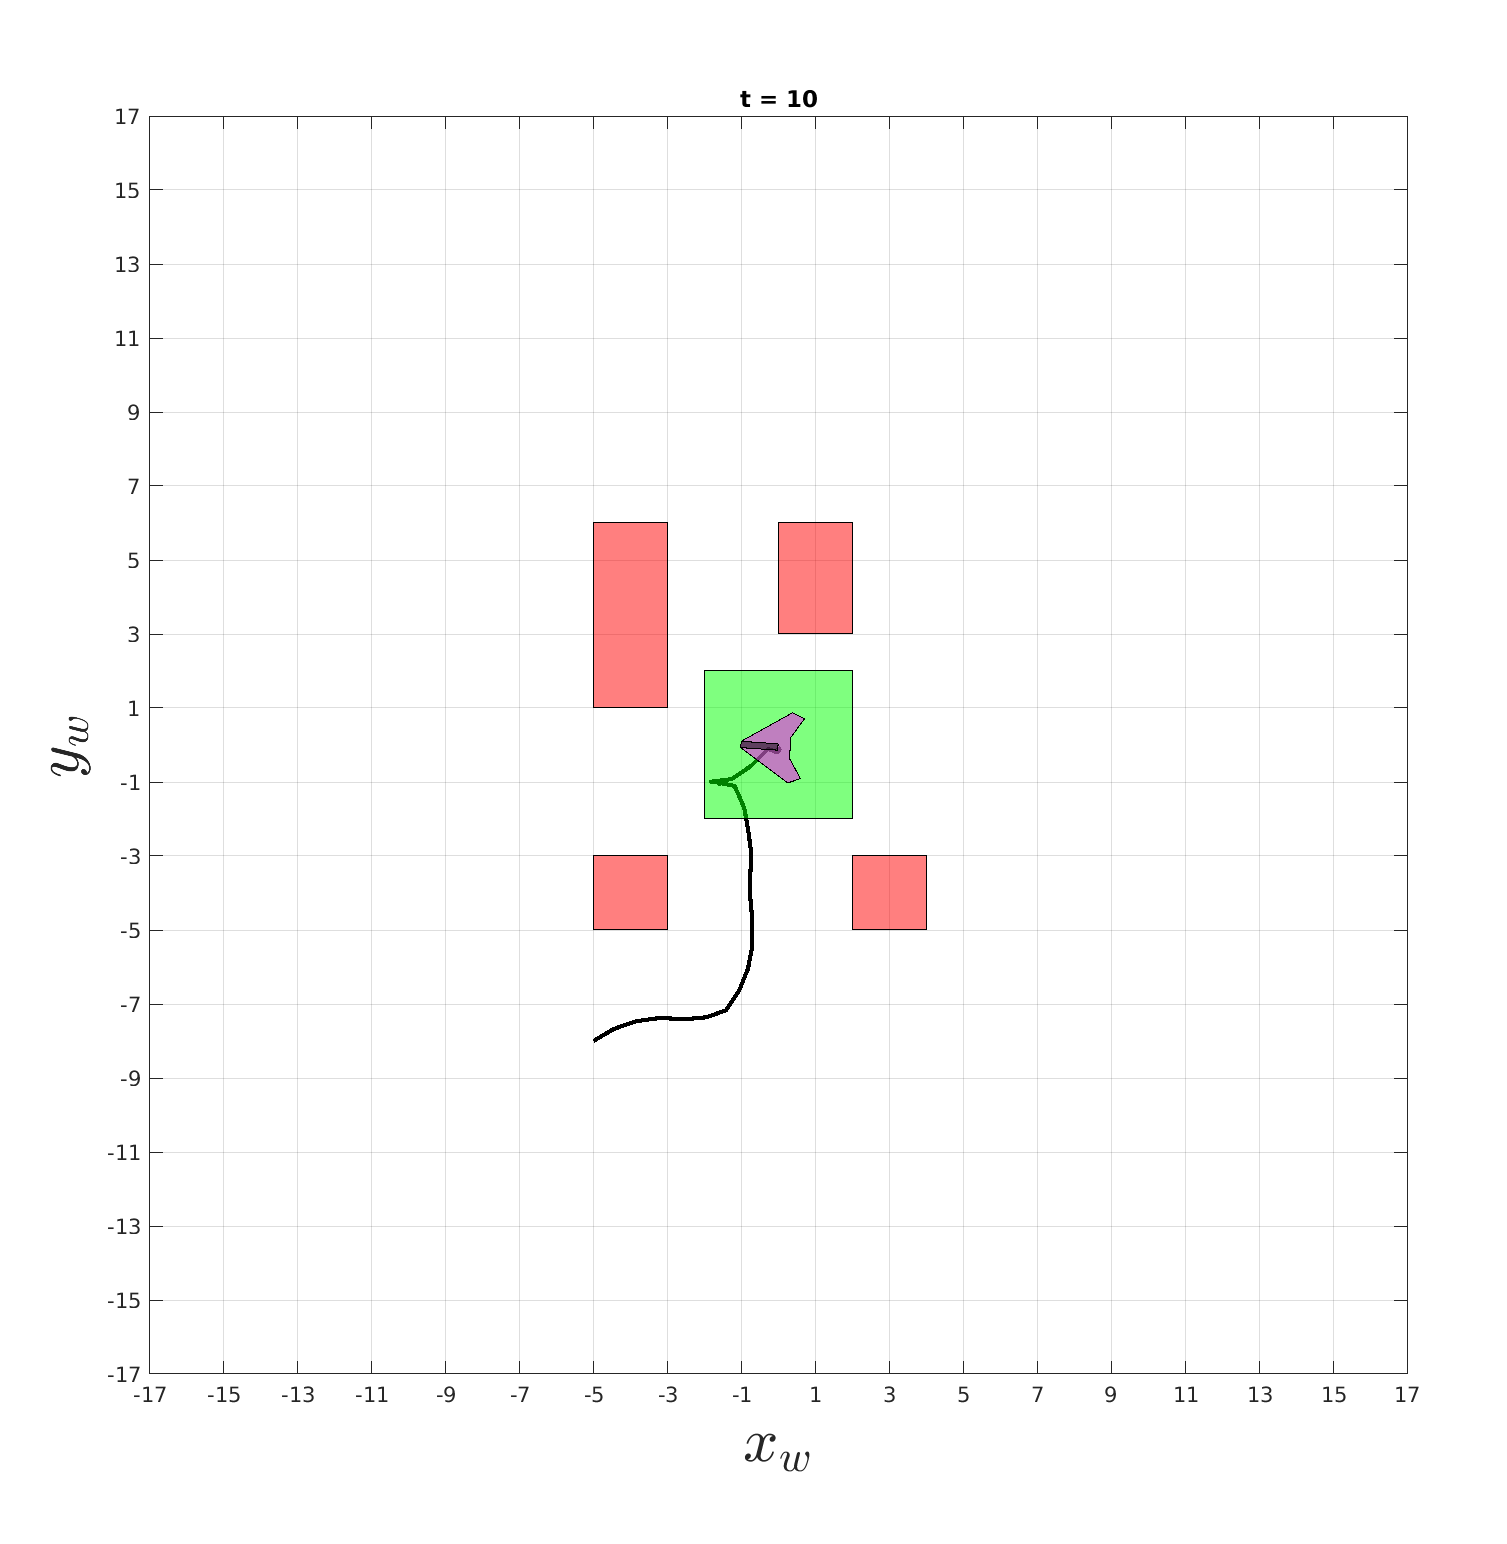
\includegraphics[scale=0.33]{figures/staticTRAJ2.png}
    So since the robot's initial position is in the limits of the $RAS$ we can see that it reaches, after the needed time, the target set in the desired angulation, avoiding the obstacles in its path. To conclude this case we can see the control inputs values playing against the optimal disturbance.
    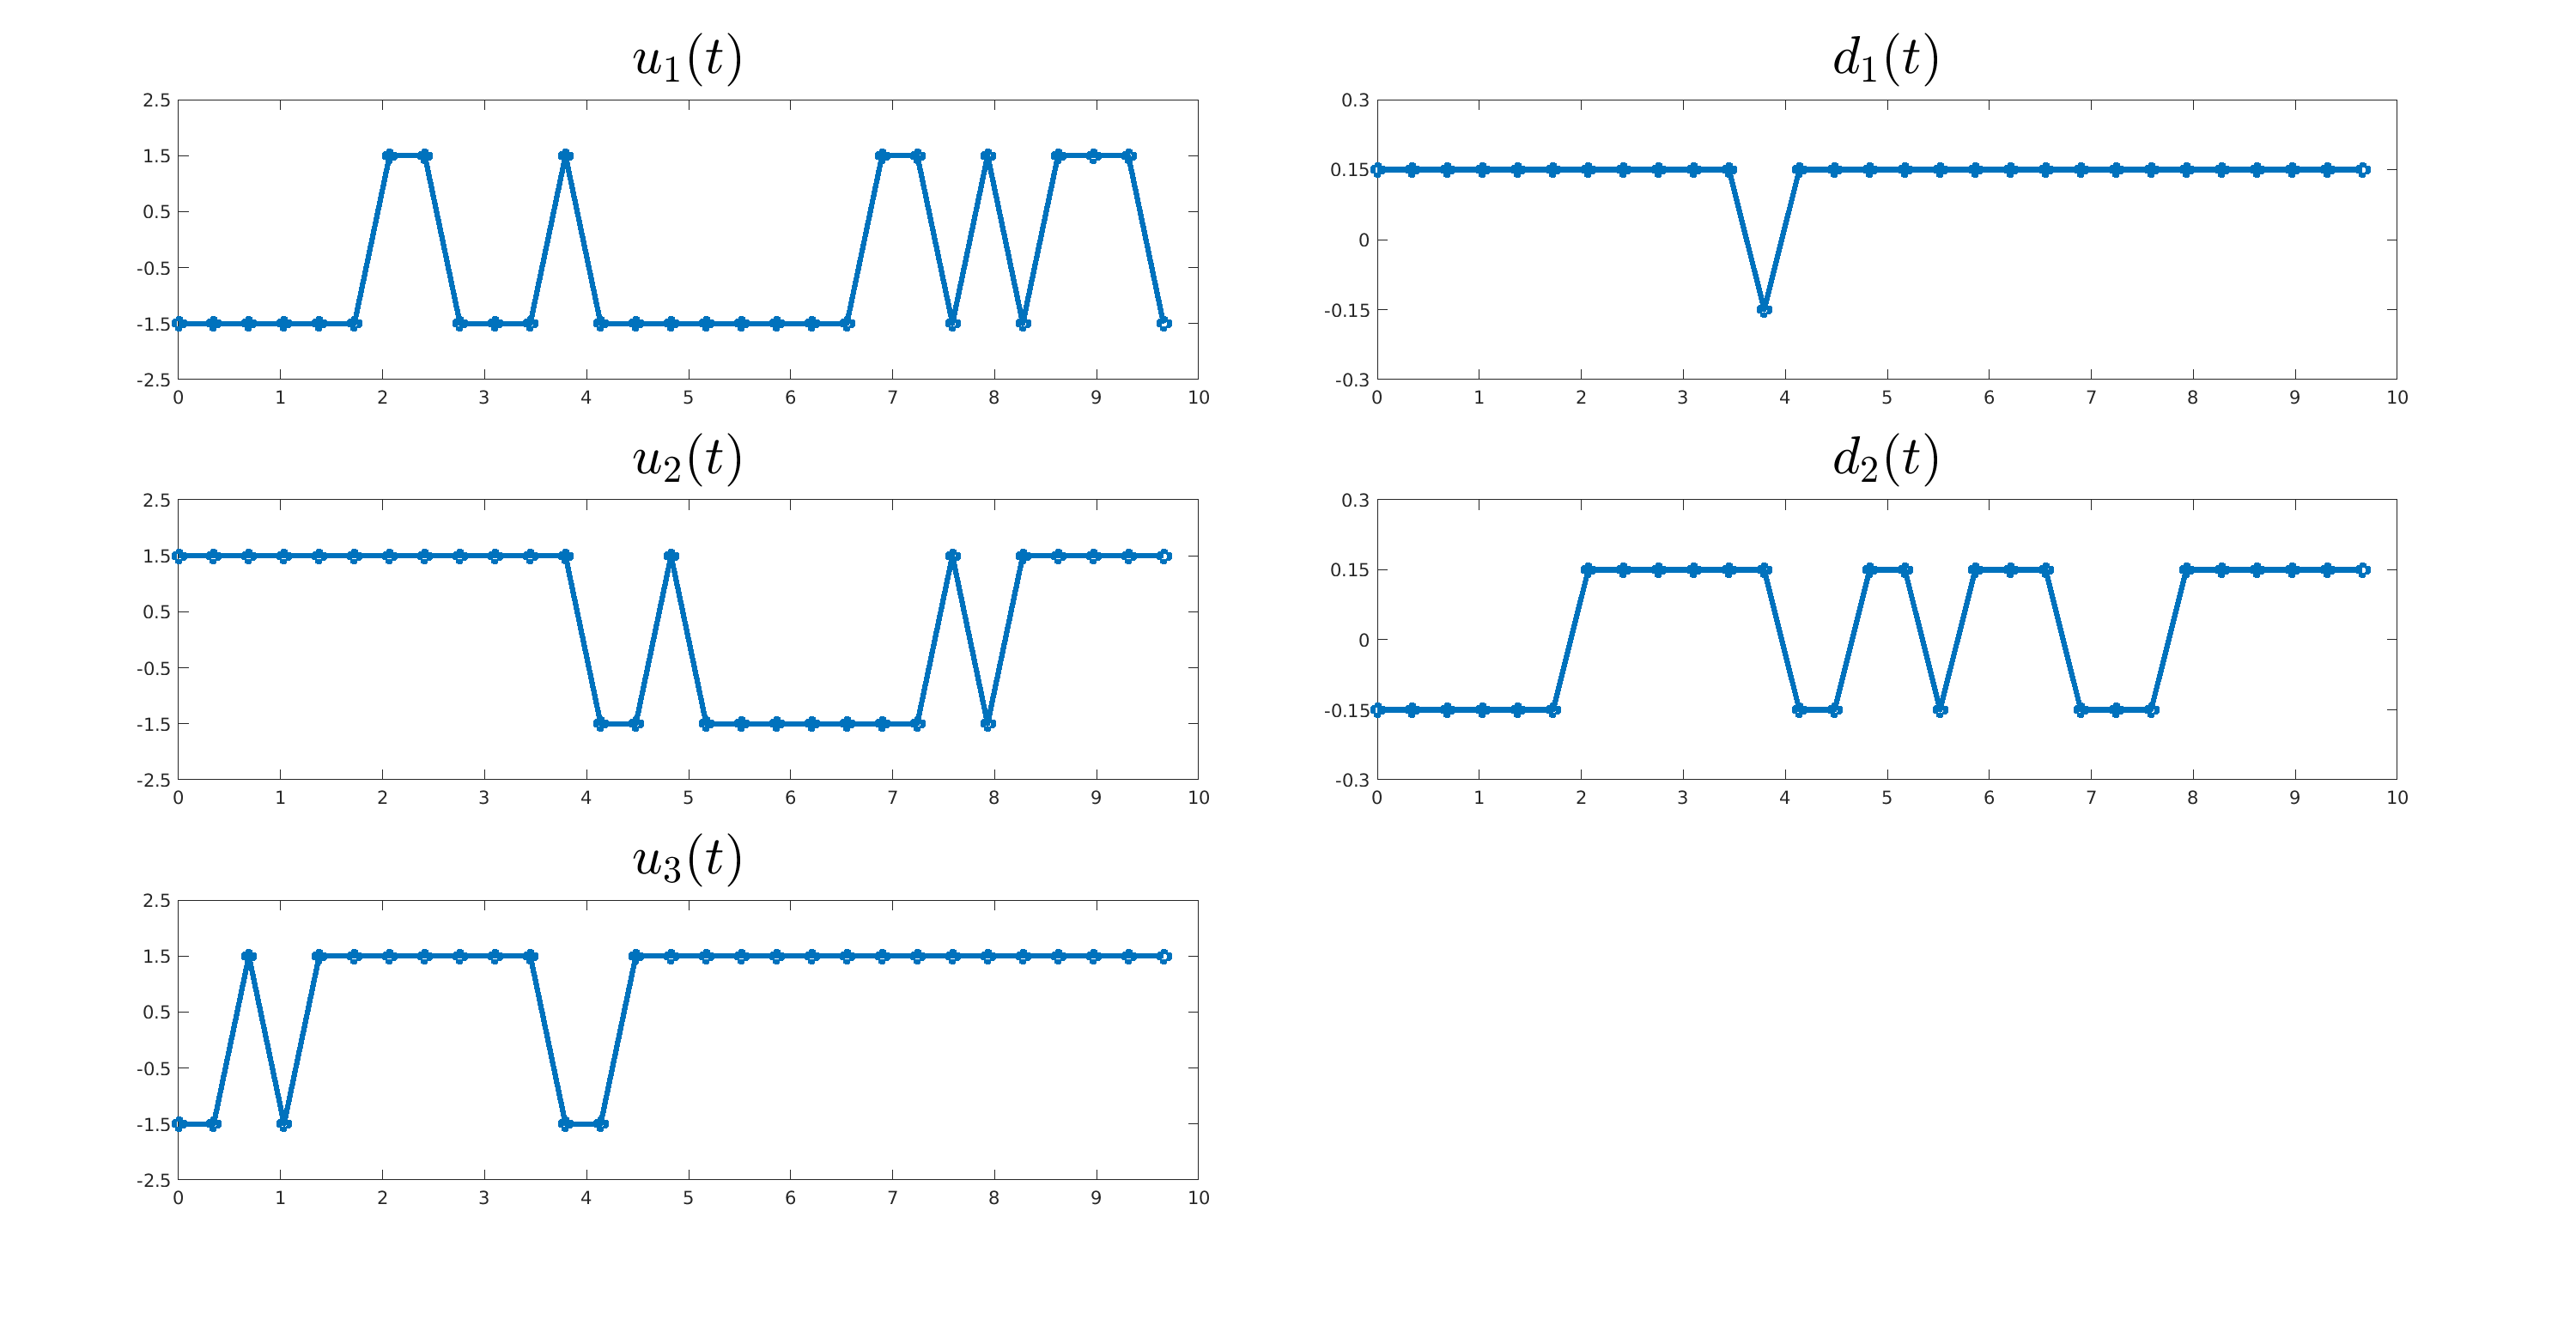
\includegraphics[scale=0.18]{figures/staticCONTROL1.png}
\subsection{Dynamic Case}
    Now we will see some more complex cases where the objects are not fixed, but they move in the environment. Here we simulated a moving platform which represent a recharging station for the robot. So the robot has to access the platform while this platform is moving downward along the Y-axis. The platform is not accessible from everywhere, but only from the right side, while the other sides are surrounded by obstacles. As mentioned before, we simulated three different cases for the Dynamic experiments. We are going to see the $RAS$ developing over time in a particular direction since the target set (always represented by a green area) is moving. The next figure represents the $RAS$ at time 10 seconds (so still not expanded). As mentioned before this represents a platform that can be entered just by one side and surrounded by obstacles. Since we are always in the configuration space we can not see the small target set which is surrounded by the red obstacles which seem bigger in the C-space.
    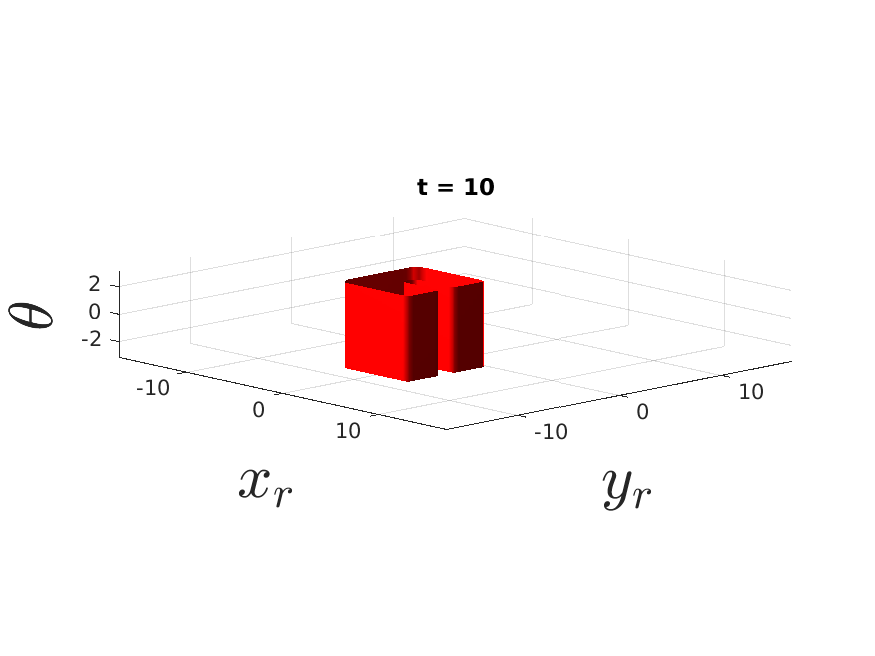
\includegraphics[scale=0.6]{figures/dynamicRAS1.png}
    At the end of the expansion of the $RAS$, so at time 0 seconds, we can see below the limits of the Set.
    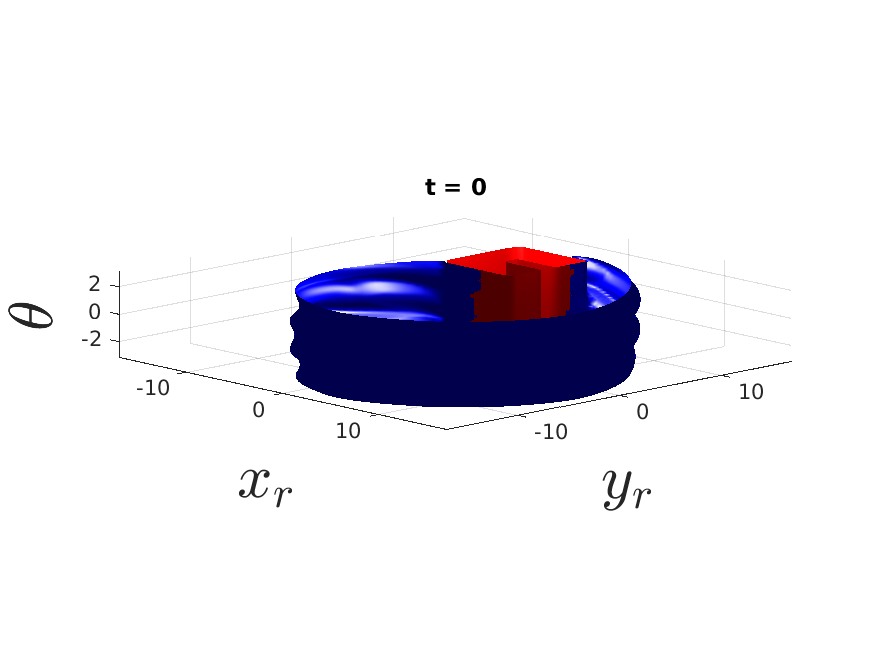
\includegraphics[scale=0.6]{figures/dynamicRAS2.png}
    We will see in each specific case a 2D representation of the $RAS$ to better understand the position of the target set and the different initial positions of the robot.
    \subsubsection{Case 1}
    In this first case the initial position of the robot is relatively near the target set and inside the $RAS$ at time 0 seconds, so we know from the theory that exists a trajectory which can lead the robot inside the target set in the maximum given time (10 seconds).
    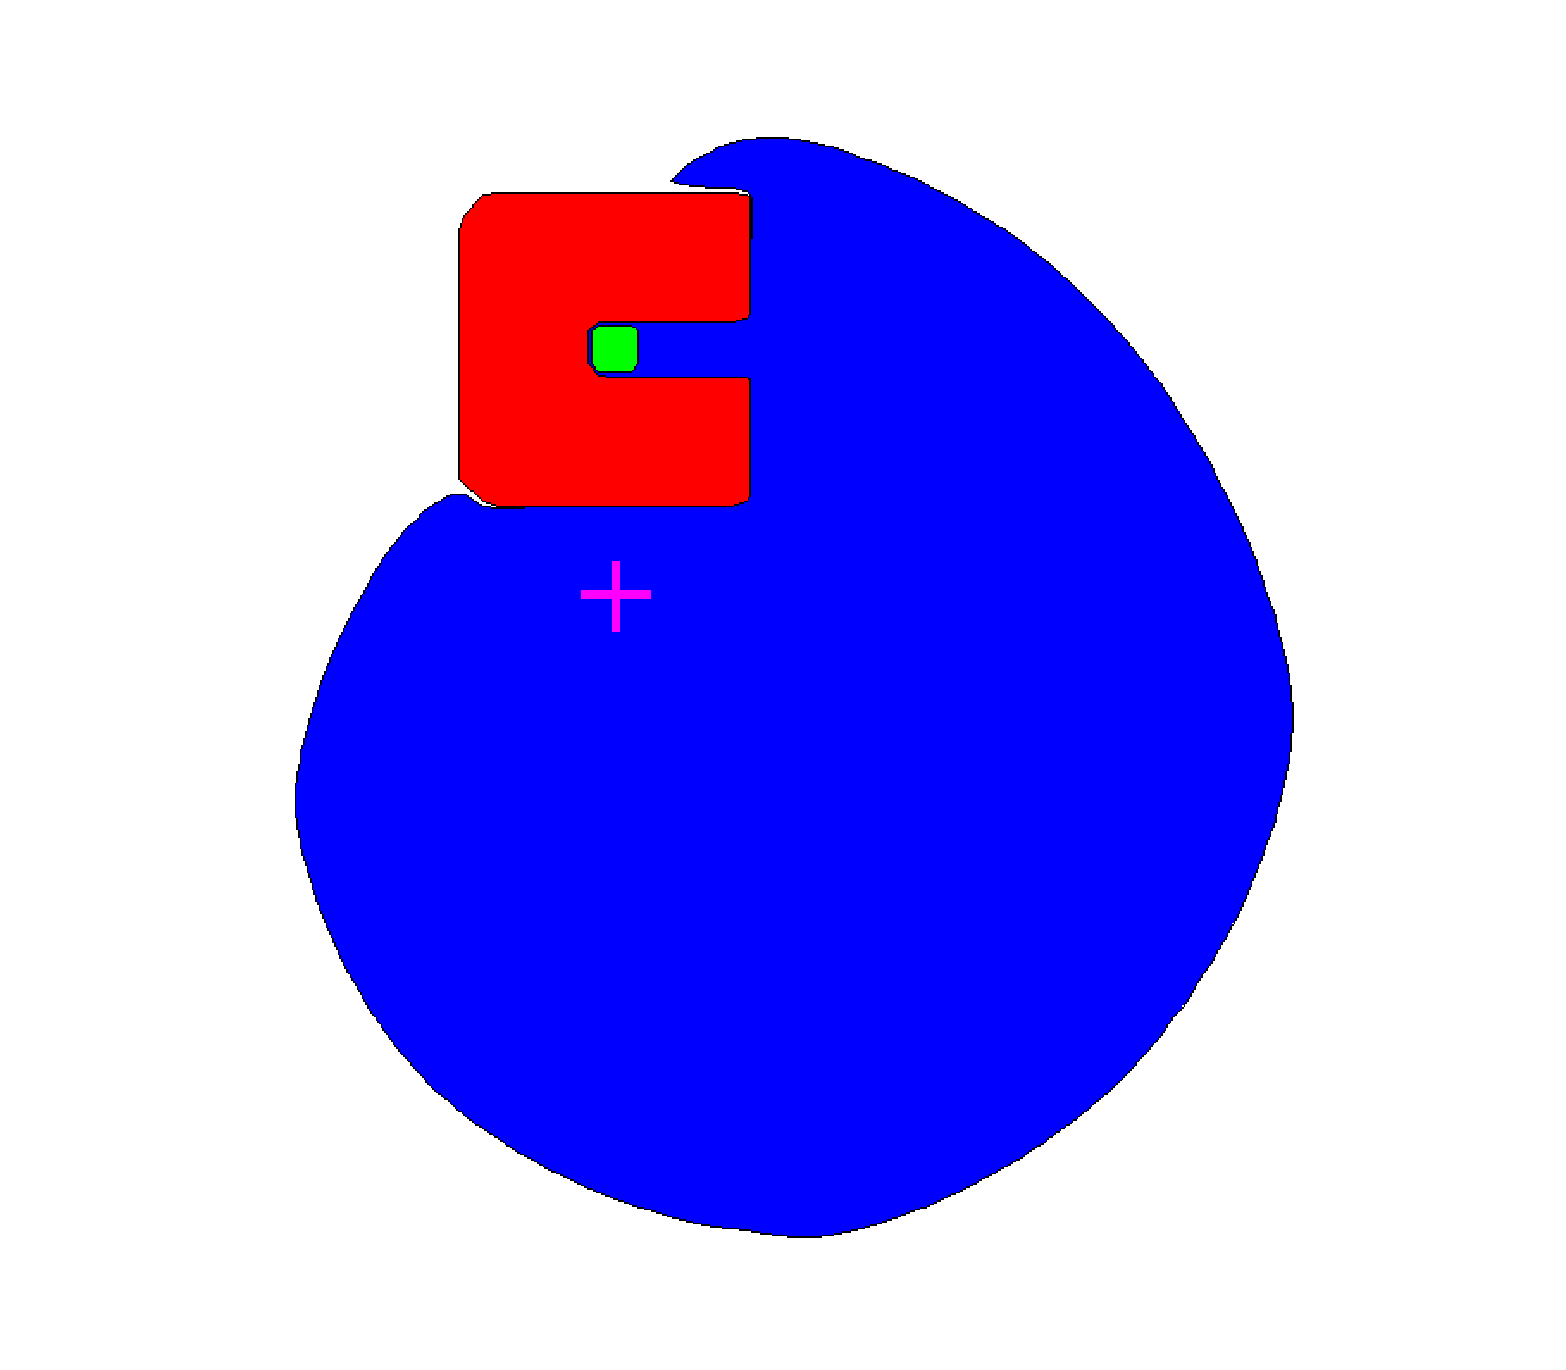
\includegraphics[scale=0.25]{figures/dynamic2Dras1.png}
    \\
    In the figure we have the 2D $RAS$ (The blue area), The obstacles (Red Area), The target set (The green area) and the initial configuration of the robot (The pink cross). From this plot we can not see the initial angular orientation of the robot since is a 2D representation, but we can better understand it from the trajectory plots below. It is important to say that the target set is not restricted only in small area of the X-axis and Y-axis , but is also limited in terms of the desired target angel $\theta$ (like in the static case). In this case we set as desired $\theta$ a small range around the angle 0 $rad$.
    \\
    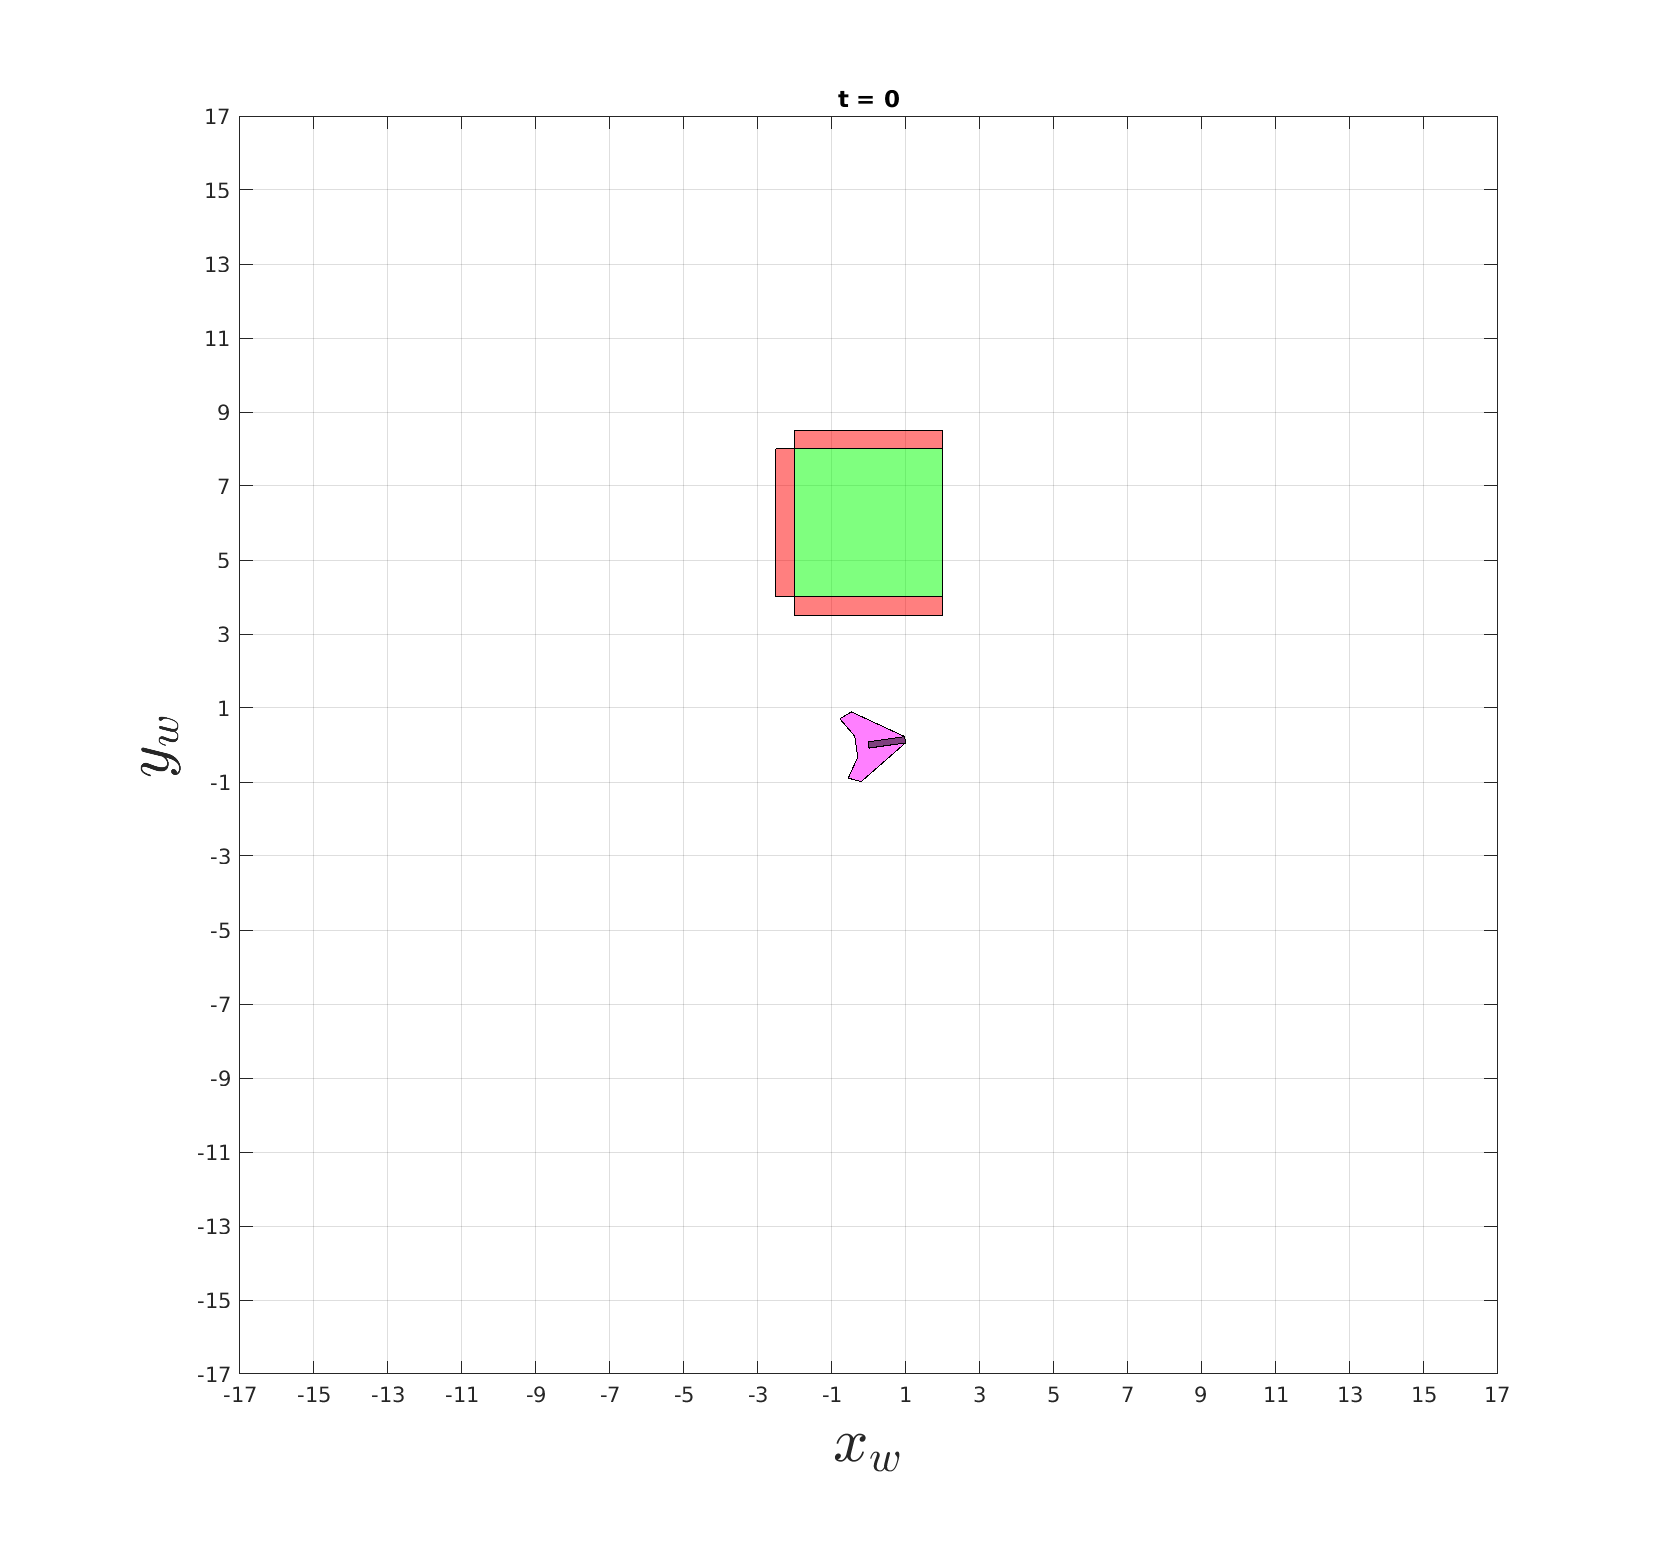
\includegraphics[scale=0.25]{figures/dynamicTRAJ1.png}
    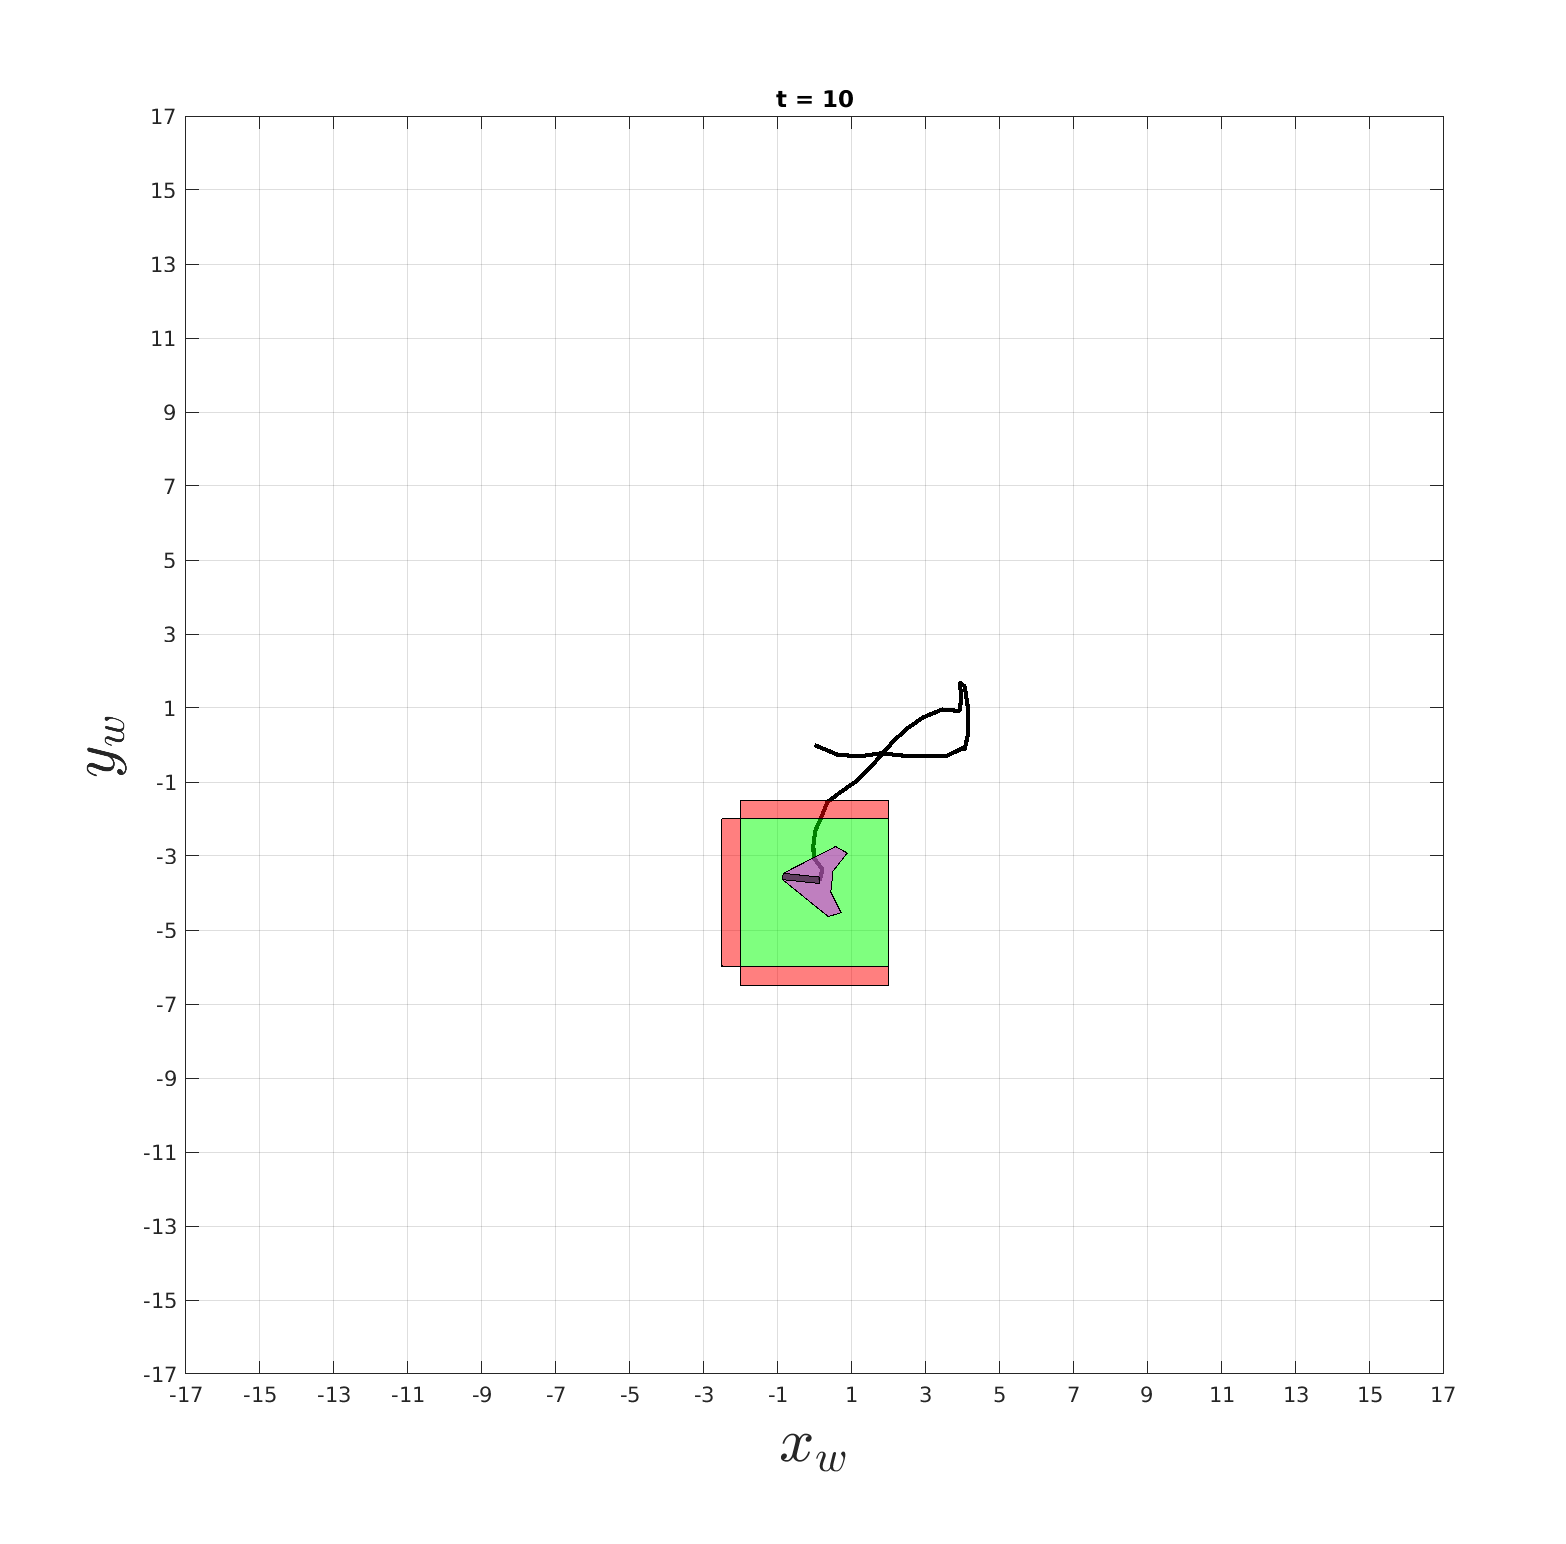
\includegraphics[scale=0.25]{figures/dynamicTRAJ2.png}
    \\
    We can see here the particular trajectory of the robot due to the movement of the target set. At time $t=10sec$ the robot is in the target set without collisions with the obstacles as expected. We can also see how it enters the target set with the desired angulation around the radiant 0
    \subsubsection{Case 2}
    The second case is similar to the previous one. In this case the only difference with the first one is the initial position of the robot. Here the robot is relatively distant from the target set, but still in the $RAS$. 
    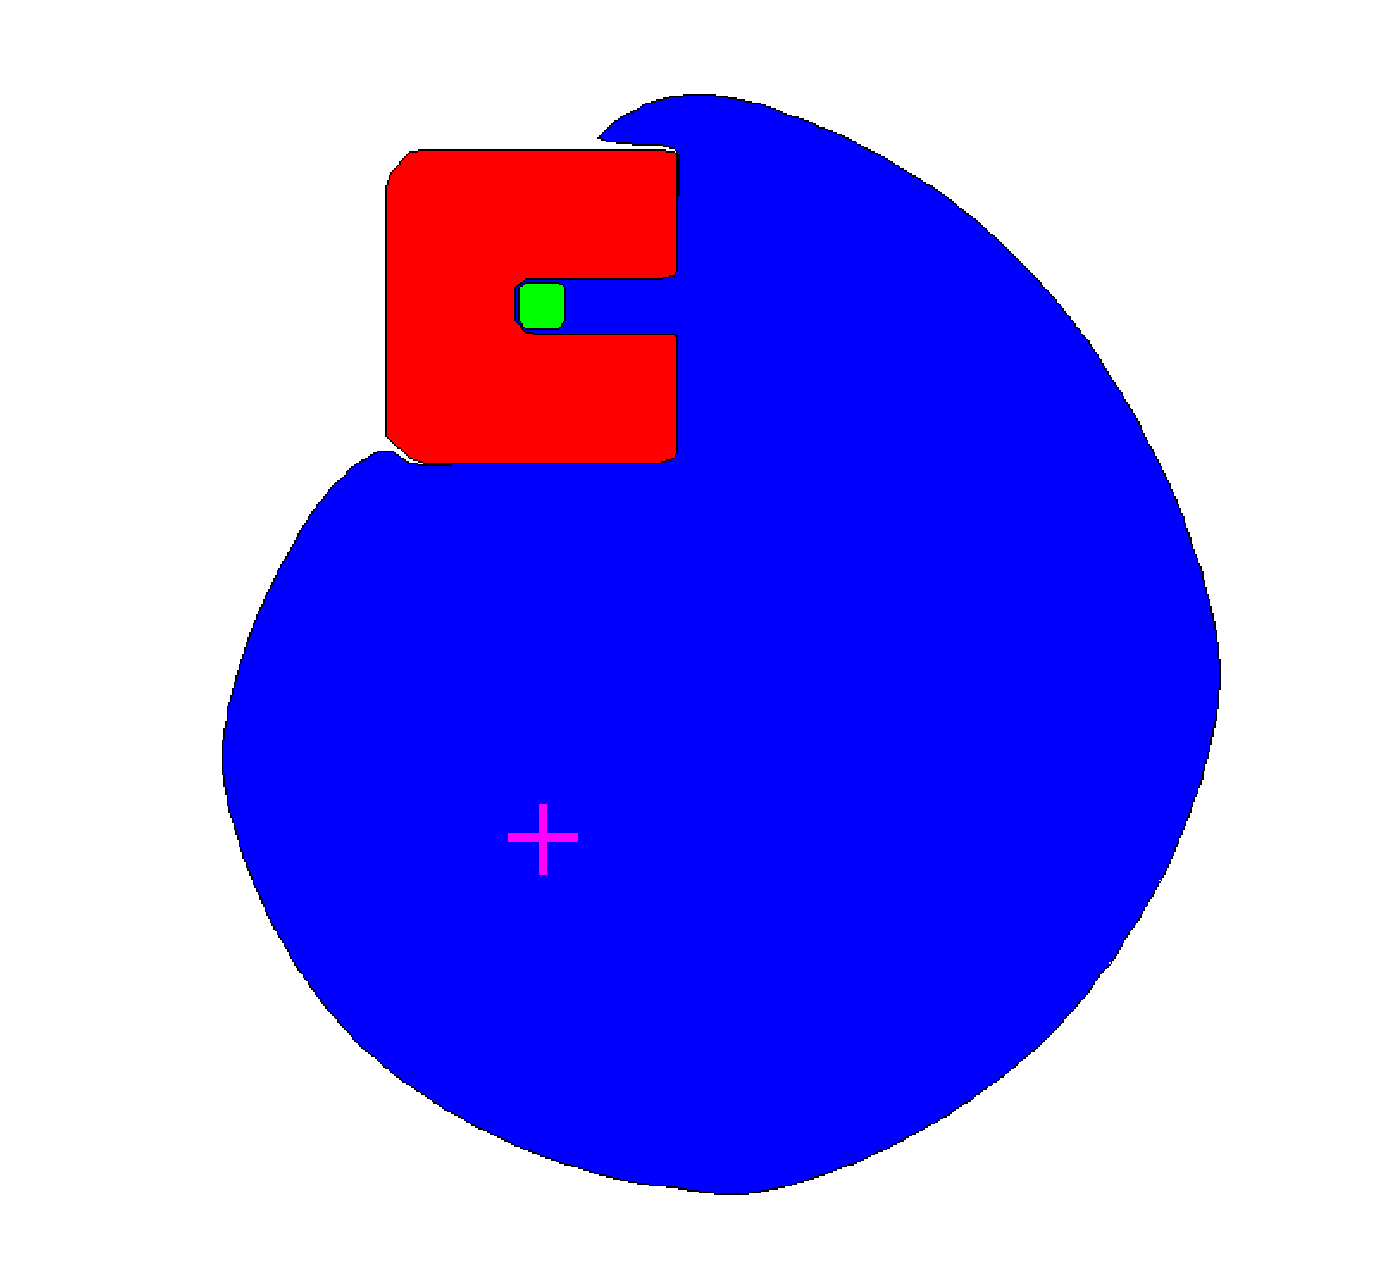
\includegraphics[scale=0.25]{figures/dynamic2Dras2.png}
    \\
    Since its initial position is still in the limits of the $RAS$ we can compute the following trajectory.
    \\
    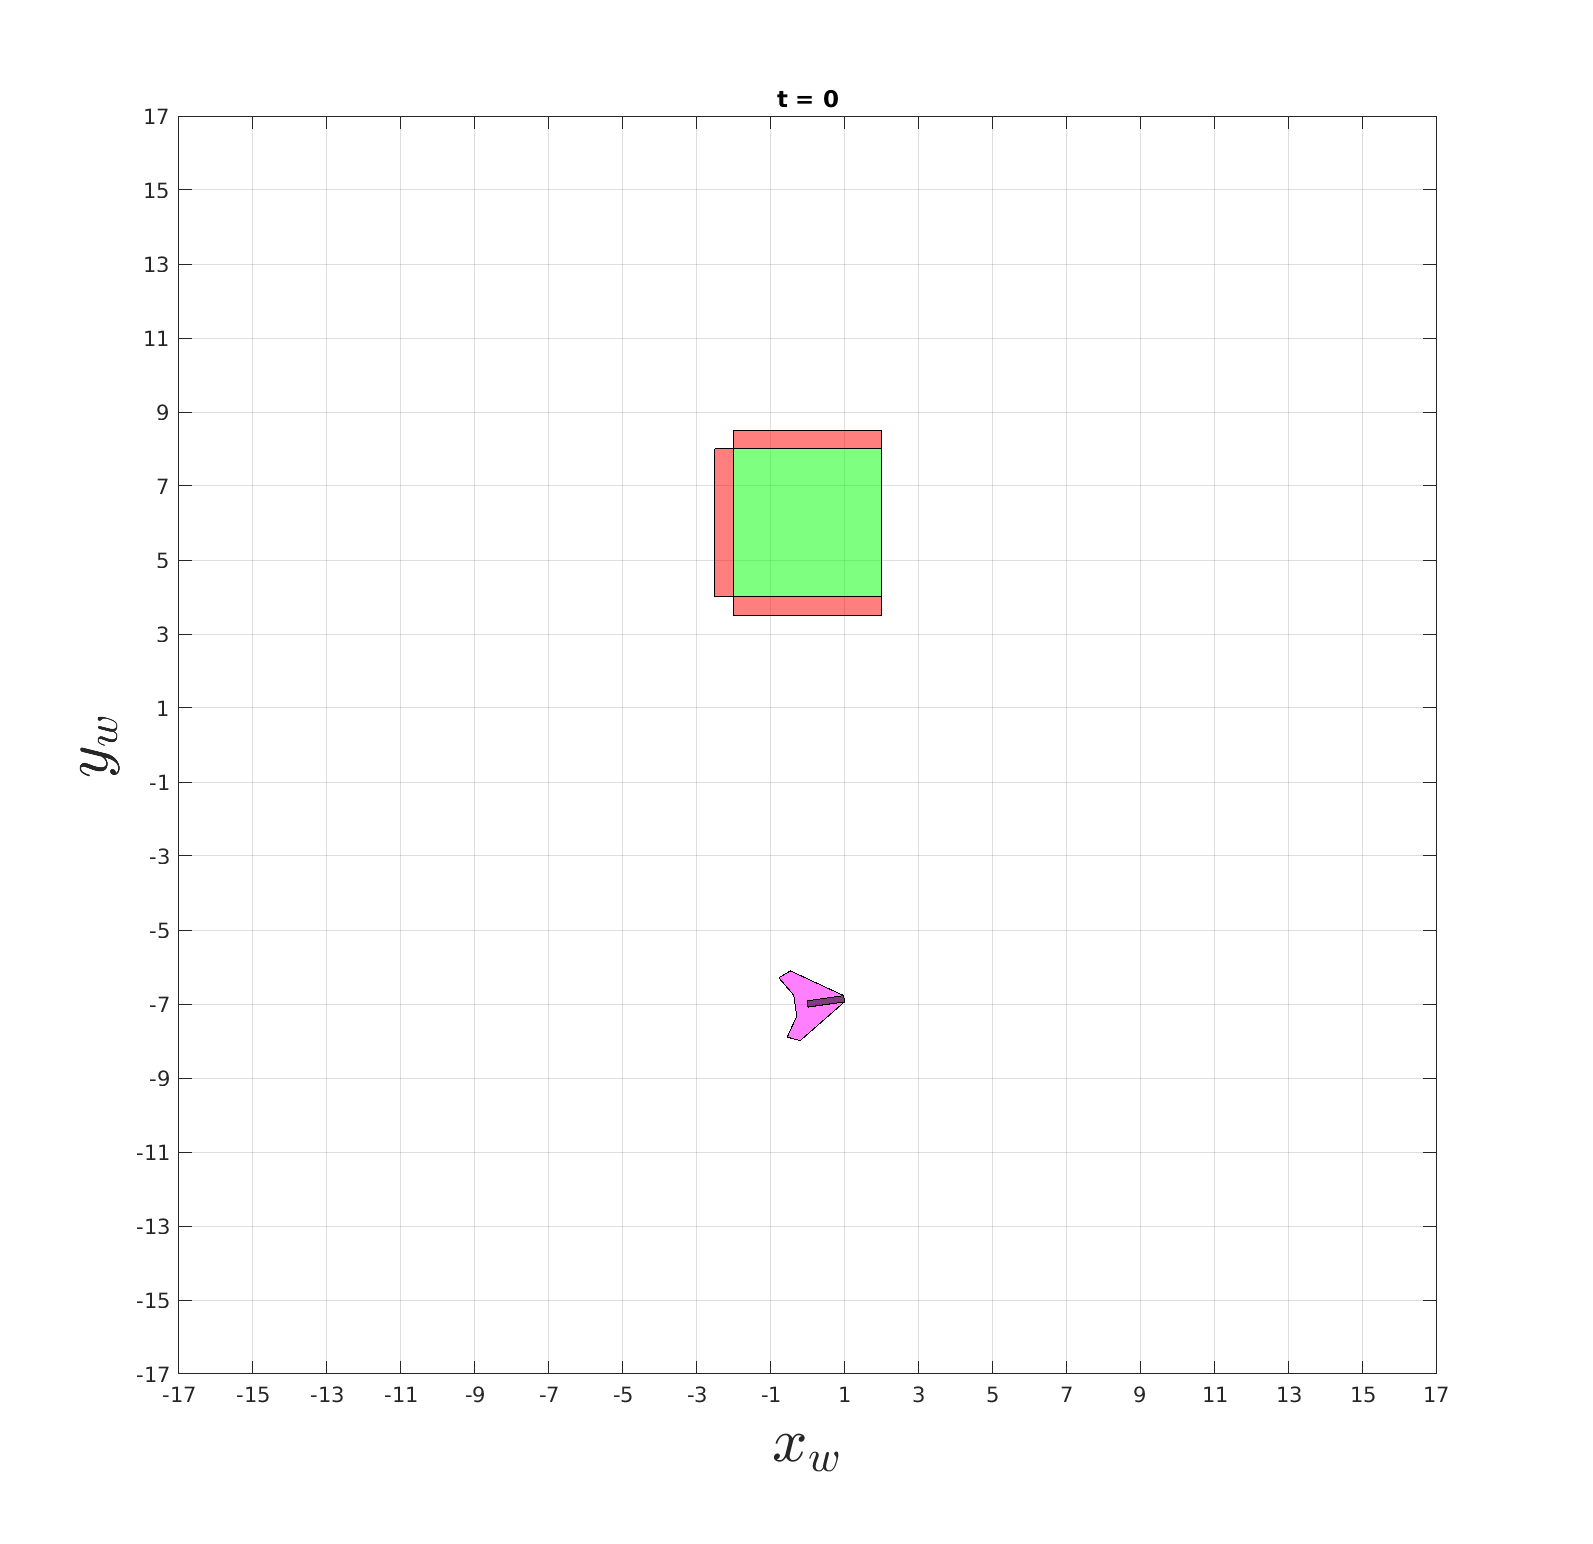
\includegraphics[scale=0.25]{figures/dynamicTRAJ3.png}
    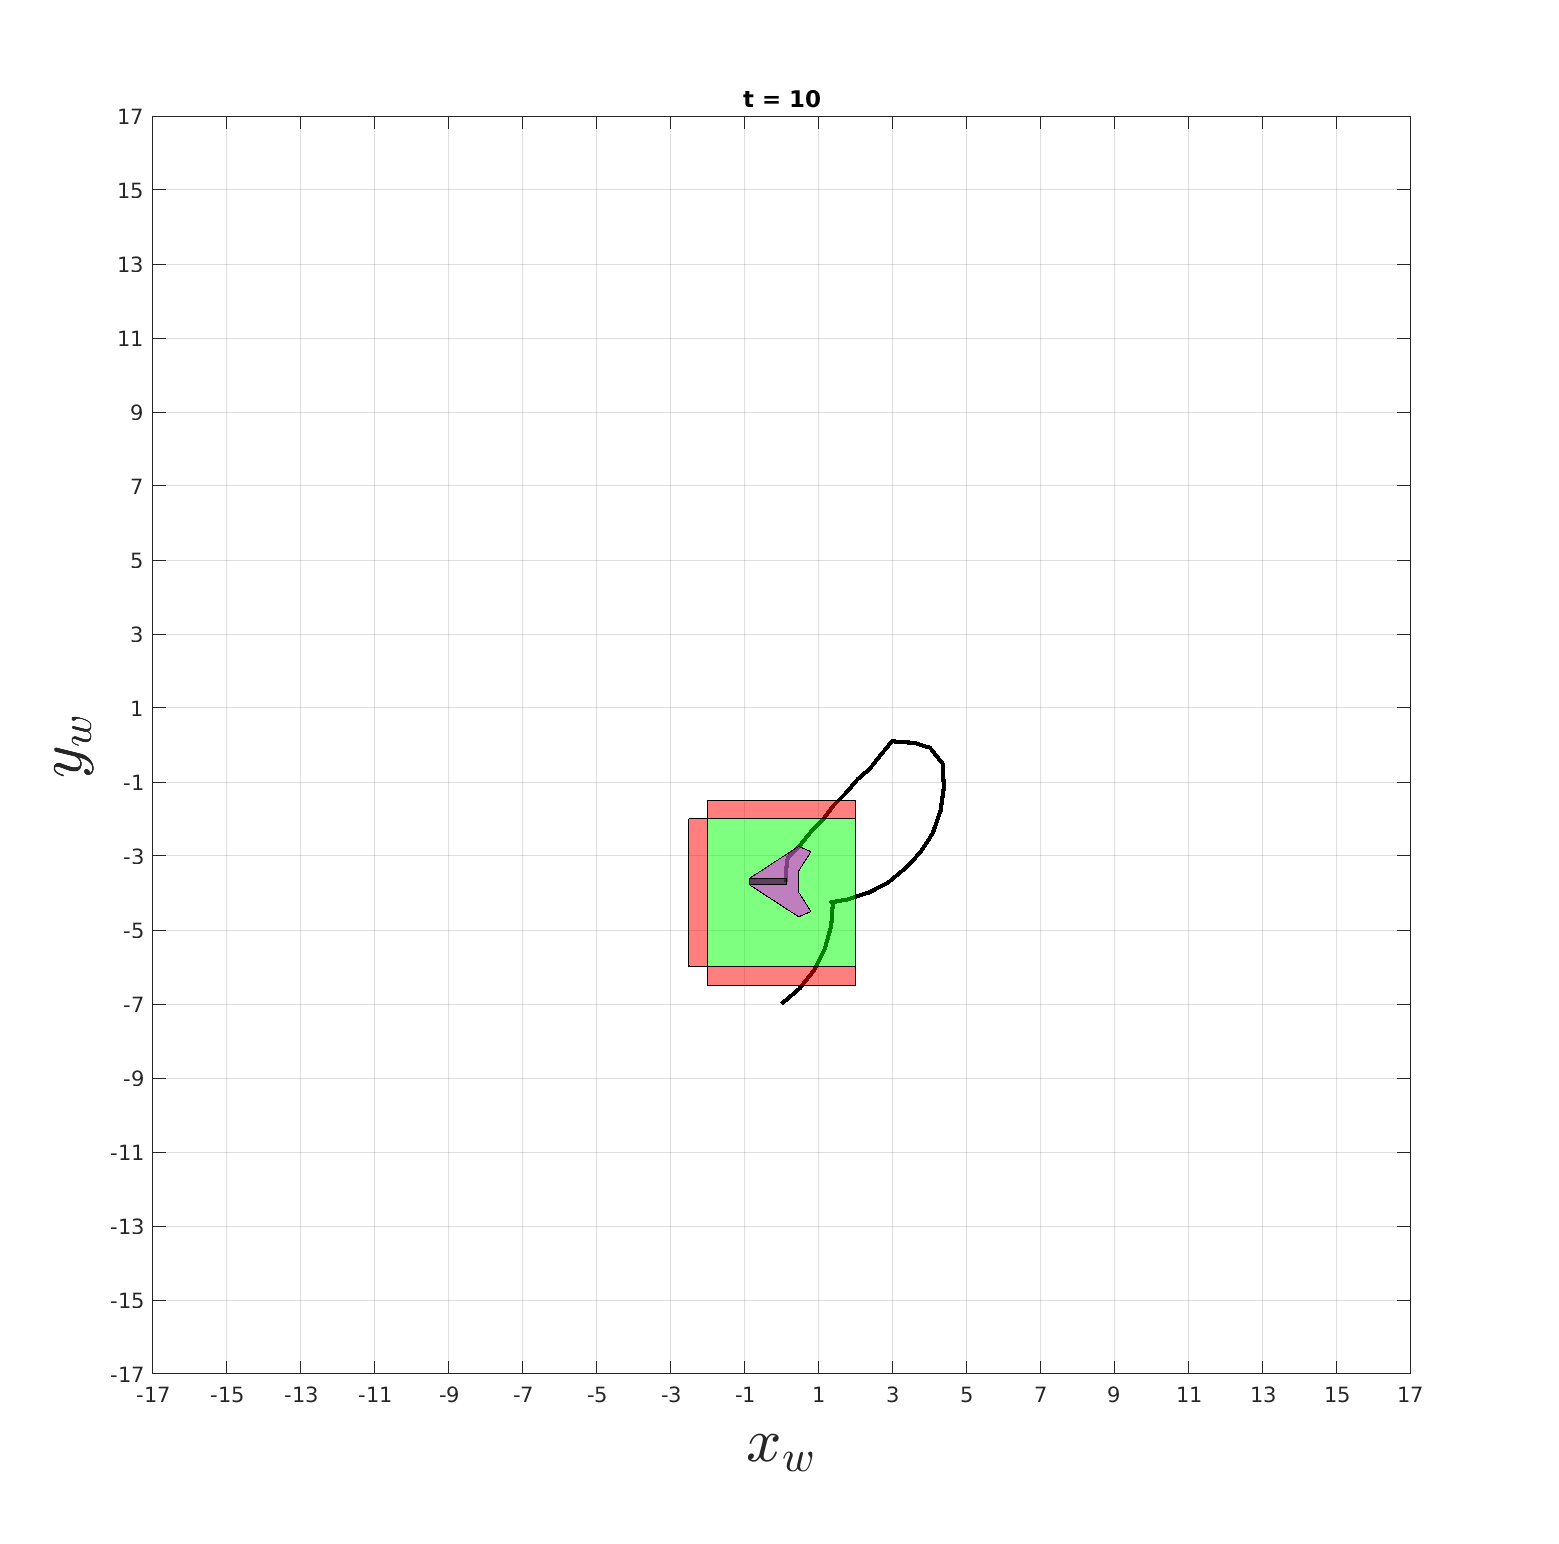
\includegraphics[scale=0.25]{figures/dynamicTRAJ4.png}
    \\
    Even in this case the Robot successfully reached the target set playing against the optimal disturbance and avoiding any obstacle.
    
    \subsubsection{Case 3}
        
        
    \section{Conclusion}
        conclusion

    \clearpage
    \appendix
        \subsection{Kinematic Model Calculation}
The three-wheeled mobile robot is used in other two papers \cite{three_wheel} \cite{motion_control} however, they do not provide the procedure to compute its kinematic model, therefore for completeness we show here the steps necessary to obtain (\ref{eq:kin_model}). The initial steps are similar to the proof shown in \cite{proof_model}.

The type of onmi-wheel used by the robot is shown in Fig.\ref{fig:omniwheel}, please notice axes of rollers are perpendicular ($90^{\circ}$) to the wheel axis, we made this clarification to avoid confusion with Mecanum wheel (a.k.a. Swedish wheel) in which axes of rollers have an angle of $45^{\circ}$, this last type is usually used in four-wheeled robot.
\begin{figure}[h]
    \centering
    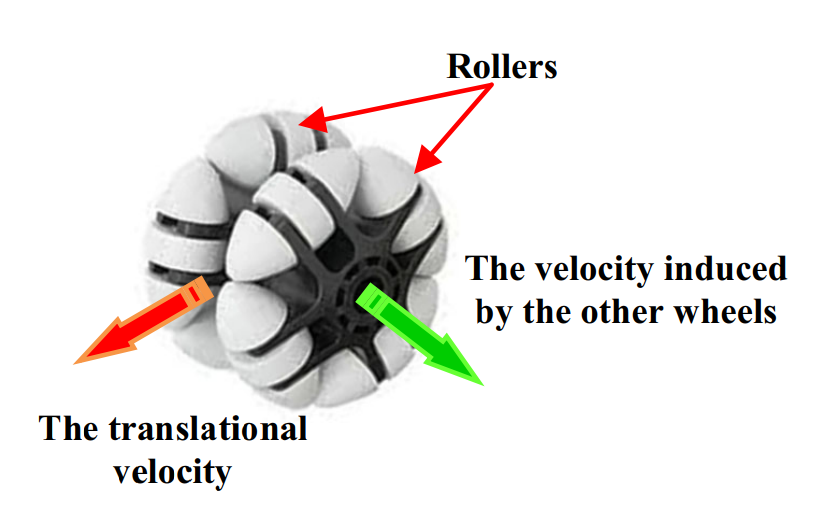
\includegraphics
        [width=0.4\textwidth]
        {figures/omniwheel.png}
    \caption{Omnidirectional wheel mounted on three-wheeled robot. Credit: \cite{proof_model}}
    \label{fig:omniwheel}
\end{figure}    
    
The first step is to compute the velocity induced to other wheels when a wheel rotates around its axis. Once computed it we can easily obtain the kinematic model w.r.t. to the robot's coordinate system $RF_m$ and then w.r.t. $RF_w$. 

\subsubsection{Induced velocity}
\begin{figure}[h]
    \centering
    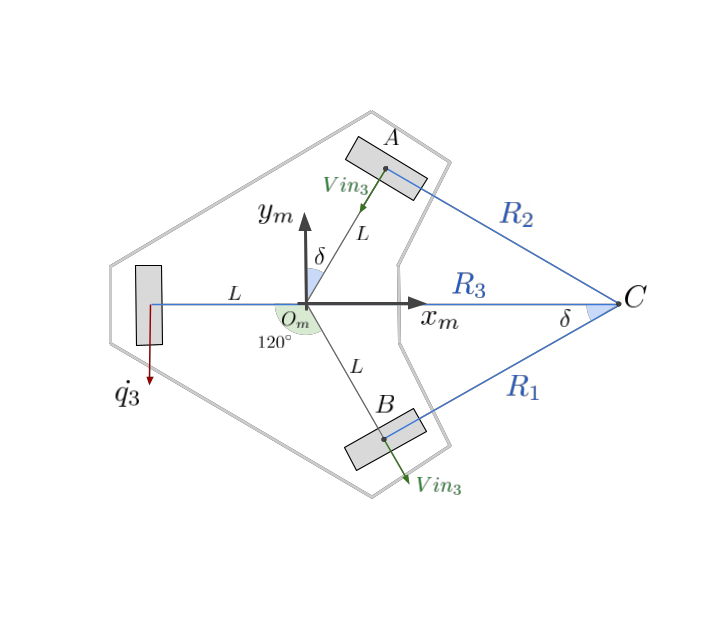
\includegraphics
        [width=0.4\textwidth]
        {figures/robot3.png}
    \caption{Induced velocity by the third wheel to the other ones}
    \label{fig:step1}
\end{figure}
Assuming that only the third wheel rotates with a velocity $\dot{q_{3}}$ and the other two wheels are inactive, we define as induced velocity $Vin_3$ the velocity that the first and second wheel gain from the third wheel. Using as reference Fig.\ref{fig:step1}, the robot turns around point $C$ with an angular velocity $\omega$ that can be expressed in two equivalent ways:
\begin{equation}
    \omega_3 = \frac{\dot{q_{3}}}{R_{3}} = \frac{V_{in3}}{R_{1}}         
    \label{omega}
\end{equation}
$R_3$ and $R_1$ can be easily computed from $\widehat{OBC}$ triangle:
\begin{equation*}
    R_3 = L + \overline{OC} = L + 2L = 3L         
\end{equation*}
\begin{equation*}
    R_1 = \frac{sin(\pi/2-\delta)}{sin(\delta)}L = \frac{cos(\delta)}{sin(\delta)}L 
\end{equation*}
Then from (\ref{omega}) we can express $Vin_3$ in terms of $\dot{q_3}$:
\begin{equation*}
    Vin_3 = \frac{R_1}{R_3}\dot{q_3}         
\end{equation*}

Due to the symmetrical mounting of the wheels, we can extend the previous result to a generic wheel $i$:

\begin{equation*}
    Vin_i = \frac{1}{3}\frac{cos(\delta)}{sin(\delta)}\dot{q_i}         
\end{equation*}

\subsubsection{Kinematic model in robot reference frame}
In the general case we have all the three wheels rotating with a specific velocity $\dot{q_{i}}$ and inducing a velocity $Vin_i$ to the others. We define a local frame $RF_i = [O_i, X_i, Y_i]$ for each wheel, $O_i$ is placed at the wheel's center, $Y_i$ is parallel to $\dot{q_i}$ and $X_i$ is placed in order to make $RF_i$ coherent with the direction of the z-axis of $RF_m$, see Fig. \ref{fig:step2}. 

\begin{figure}[h]
    \centering
    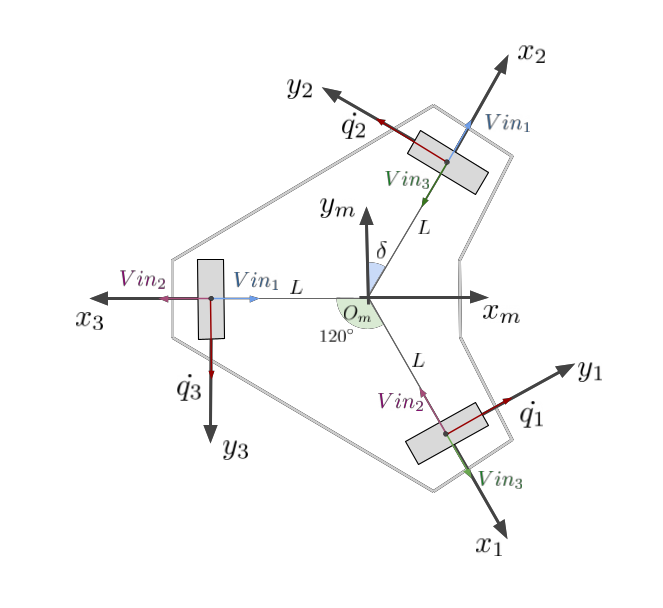
\includegraphics
        [width=0.4\textwidth]
        {figures/robot4.png}
    \caption{Resulting velocities w.r.t. $RF_i$}
    \label{fig:step2}
\end{figure}

The resulting velocities of each wheel $i$ w.r.t to $RF_i$ are the following:
\begin{gather}
    ^1V_1 =
    \begin{pmatrix} 
        Vin_3-Vin_2 \\
        \dot{q_{1}}
    \end{pmatrix}
    \\
    ^2V_2 =
    \begin{pmatrix} 
        Vin_1-Vin_3 \\
        \dot{q_{2}}
    \end{pmatrix}
    \\
    ^3V_3 =
    \begin{pmatrix} 
        Vin_2-Vin_1 \\
        \dot{q_{3}}
    \end{pmatrix}
\end{gather}
We can rewrite each of them w.r.t. $RF_m$ using:
\begin{equation*}
    ^mV_1 =\, ^mR_1\,^1V_1, \quad ^mV_2 =\, ^mR_2\, ^2V_2,\quad  ^mV_3 =\, ^mR_3\,  ^3V_3
\end{equation*}
Where:
\begin{equation*}
    ^mR_1 = R_{z}\left(-\frac{\pi}{2}+\delta\right), \, ^mR_2 = R_{z}\left(\frac{\pi}{2}-\delta\right), \, ^mR_3 = R_{z}\left(\pi\right)
\end{equation*}
\begin{equation*}
    R_{z}(\alpha) = \begin{pmatrix}
                \cos(\alpha) & -\sin(\alpha)\\
                \sin(\alpha) & \cos(\alpha)
            \end{pmatrix}
\end{equation*}

The whole angular velocity of the robot can be obtained by summing each single contribution $\omega_i$ (\ref{omega}):
\begin{equation*}
    \omega = \omega_1 + \omega_2 + \omega_3 
\end{equation*}
Therefore, the kinematic model w.r.t. the $RF_{m}$ is given by:
\begin{equation}
    \left\{
        \begin{array}{ll}
            \begin{pmatrix} 
                \dot{^m x_r} \\ 
                ^m y_r  
            \end{pmatrix} 
            = \frac
                {^m V_1 + ^m V_2 + ^m V_3}
                {3}\\
            
            \omega = \frac{1}{3L}\left(\dot{q_{1}} + \dot{q_{2}} + \dot{q_{3}}\right)
        \end{array}
    \right.
    \label{robot_ref}
\end{equation}

\subsubsection{Model in the world coordinate system}
Finally, starting from (\ref{robot_ref}), we can compute the kinematic model w.r.t to the world reference frame $RF_w$. The angular velocity remains the same, for the position we use a rotation around z-axis:

\begin{equation}
	\label{world_ref}
	\left\{
		\begin{array}{ll}
			\dot{^w x_r} = R_z(\theta)\, \dot{^m x_r}\\
			\dot{^w y_r} = R_z(\theta)\, \dot{^m y_r}\\
            \dot{\theta} = \omega
		\end{array}
	\right.
\end{equation}

Carrying out the calculations with $\delta=30^{\circ}$, from (\ref{world_ref}) we obtain (\ref{eq:kin_model}). \footnote{Matlab notebook \textit{proof\_model.mlx} in code folder shows the computation}


    \begin{thebibliography}{1}

%\bibitem{example}
%N. Surname, ``Paper's name'',
%\emph{source / where it can be found}.

\bibitem{brief_intro}
S. Bansal, Mo Chen, S. Herbert and C. J. Tomlin, ``Hamilton-Jacobi Reachability: A Brief Overview and Recent Advances'',
\emph{arxiv.org/abs/1709.07523}.

\bibitem{reach_avoid_no_dist}
K. Margellos and J. Lygeros, ``Hamilton-Jacobi formulation for reach-avoid problems with an application to air traffic management'',
\emph{Proceedings of the 2010 American Control Conference}, 2010, pp. 3045-3050, doi: 10.1109/ACC.2010.5530514.

\bibitem{reach_avoid_with_dist}
K. Margellos and J. Lygeros, ``Hamilton–Jacobi Formulation for Reach–Avoid Differential Games,''
\emph{in IEEE Transactions on Automatic Control}, vol. 56, no. 8, pp. 1849-1861, Aug. 2011, doi: 10.1109/TAC.2011.2105730.

\bibitem{three_wheel}
Datar, Mandar \& Ketkar, Vishwanath \& Mejari, Manas \& Gupta, Ankit \& Singh, N.M. \& Kazi, Faruk, ``Motion Planning for the Three Wheel Mobile Robot using the Reachable Set Computation under Constraints, (2014)''
\emph{IFAC Proceedings Volumes (IFAC-PapersOnline)}, 3. 10.3182/20140313-3-IN-3024.00178.

\bibitem{mitchell_time_dep_HJ}
I. M. Mitchell, A. M. Bayen and C. J. Tomlin, ``A time-dependent Hamilton-Jacobi formulation of reachable sets for continuous dynamic games,''
\emph{in IEEE Transactions on Automatic Control}, vol. 50, no. 7, pp. 947-957, July 2005, doi: 10.1109/TAC.2005.851439.

\bibitem{evans}
Lawrence C. Evans and Panagiotis E. Souganidis, ``Differential Games and Representation Formulas for Solutions of Hamilton-Jacobi-Isaacs Equations'',
\emph{Indiana University Mathematics Journal (1983), volume 33, pages 773-797}.

\bibitem{new_paper}
Fisac, Jaime, Chen, Mo, Tomlin, Claire, Sastry, Shankar, ``Reach-Avoid Problems with Time-Varying Dynamics, Targets and Constraints (2014)'',
\emph{https://arxiv.org/abs/1410.6445}.

\end{thebibliography}

\end{document}